\documentclass[twoside]{book}

% Packages required by doxygen
\usepackage{fixltx2e}
\usepackage{calc}
\usepackage{doxygen}
\usepackage[export]{adjustbox} % also loads graphicx
\usepackage{graphicx}
\usepackage[utf8]{inputenc}
\usepackage{makeidx}
\usepackage{multicol}
\usepackage{multirow}
\PassOptionsToPackage{warn}{textcomp}
\usepackage{textcomp}
\usepackage[nointegrals]{wasysym}
\usepackage[table]{xcolor}

% Font selection
\usepackage[T1]{fontenc}
\usepackage[scaled=.90]{helvet}
\usepackage{courier}
\usepackage{amssymb}
\usepackage{sectsty}
\renewcommand{\familydefault}{\sfdefault}
\allsectionsfont{%
  \fontseries{bc}\selectfont%
  \color{darkgray}%
}
\renewcommand{\DoxyLabelFont}{%
  \fontseries{bc}\selectfont%
  \color{darkgray}%
}
\newcommand{\+}{\discretionary{\mbox{\scriptsize$\hookleftarrow$}}{}{}}

% Page & text layout
\usepackage{geometry}
\geometry{%
  a4paper,%
  top=2.5cm,%
  bottom=2.5cm,%
  left=2.5cm,%
  right=2.5cm%
}
\tolerance=750
\hfuzz=15pt
\hbadness=750
\setlength{\emergencystretch}{15pt}
\setlength{\parindent}{0cm}
\setlength{\parskip}{3ex plus 2ex minus 2ex}
\makeatletter
\renewcommand{\paragraph}{%
  \@startsection{paragraph}{4}{0ex}{-1.0ex}{1.0ex}{%
    \normalfont\normalsize\bfseries\SS@parafont%
  }%
}
\renewcommand{\subparagraph}{%
  \@startsection{subparagraph}{5}{0ex}{-1.0ex}{1.0ex}{%
    \normalfont\normalsize\bfseries\SS@subparafont%
  }%
}
\makeatother

% Headers & footers
\usepackage{fancyhdr}
\pagestyle{fancyplain}
\fancyhead[LE]{\fancyplain{}{\bfseries\thepage}}
\fancyhead[CE]{\fancyplain{}{}}
\fancyhead[RE]{\fancyplain{}{\bfseries\leftmark}}
\fancyhead[LO]{\fancyplain{}{\bfseries\rightmark}}
\fancyhead[CO]{\fancyplain{}{}}
\fancyhead[RO]{\fancyplain{}{\bfseries\thepage}}
\fancyfoot[LE]{\fancyplain{}{}}
\fancyfoot[CE]{\fancyplain{}{}}
\fancyfoot[RE]{\fancyplain{}{\bfseries\scriptsize Generated by Doxygen }}
\fancyfoot[LO]{\fancyplain{}{\bfseries\scriptsize Generated by Doxygen }}
\fancyfoot[CO]{\fancyplain{}{}}
\fancyfoot[RO]{\fancyplain{}{}}
\renewcommand{\footrulewidth}{0.4pt}
\renewcommand{\chaptermark}[1]{%
  \markboth{#1}{}%
}
\renewcommand{\sectionmark}[1]{%
  \markright{\thesection\ #1}%
}

% Indices & bibliography
\usepackage{natbib}
\usepackage[titles]{tocloft}
\setcounter{tocdepth}{3}
\setcounter{secnumdepth}{5}
\makeindex

% Hyperlinks (required, but should be loaded last)
\usepackage{ifpdf}
\ifpdf
  \usepackage[pdftex,pagebackref=true]{hyperref}
\else
  \usepackage[ps2pdf,pagebackref=true]{hyperref}
\fi
\hypersetup{%
  colorlinks=true,%
  linkcolor=blue,%
  citecolor=blue,%
  unicode%
}

% Custom commands
\newcommand{\clearemptydoublepage}{%
  \newpage{\pagestyle{empty}\cleardoublepage}%
}

\usepackage{caption}
\captionsetup{labelsep=space,justification=centering,font={bf},singlelinecheck=off,skip=4pt,position=top}

%===== C O N T E N T S =====

\begin{document}

% Titlepage & ToC
\hypersetup{pageanchor=false,
             bookmarksnumbered=true,
             pdfencoding=unicode
            }
\pagenumbering{roman}
\begin{titlepage}
\vspace*{7cm}
\begin{center}%
{\Large vinecopulib \\[1ex]\large 0.\+0.\+1.\+9990 }\\
\vspace*{1cm}
{\large Generated by Doxygen 1.8.11}\\
\end{center}
\end{titlepage}
\clearemptydoublepage
\tableofcontents
\clearemptydoublepage
\pagenumbering{arabic}
\hypersetup{pageanchor=true}

%--- Begin generated contents ---
\chapter{vinecopulib\+: a C++ library for vine copula modeling}
\label{index}\hypertarget{index}{}\begin{DoxyAuthor}{Authors}
Thomas Nagler and Thibault Vatter
\end{DoxyAuthor}
This is the A\+PI documentation for the vinecopulib C++ library. It provides functionality for statistical dependence modeling with bivariate and vine copulas. For a more high-\/level overview see \href{https://github.com/tvatter/vinecopulib/blob/master/README.md}{\tt R\+E\+A\+D\+ME}.\hypertarget{index_license}{}\section{License}\label{index_license}
The M\+IT License (M\+IT)

Copyright © 2017 Thibault Vatter and Thomas Nagler

Permission is hereby granted, free of charge, to any person obtaining a copy of this software and associated documentation files (the “\+Software”), to deal in the Software without restriction, including without limitation the rights to use, copy, modify, merge, publish, distribute, sublicense, and/or sell copies of the Software, and to permit persons to whom the Software is furnished to do so, subject to the following conditions\+:

The above copyright notice and this permission notice shall be included in all copies or substantial portions of the Software.

T\+HE S\+O\+F\+T\+W\+A\+RE IS P\+R\+O\+V\+I\+D\+ED “\+AS I\+S”, W\+I\+T\+H\+O\+UT W\+A\+R\+R\+A\+N\+TY OF A\+NY K\+I\+ND, E\+X\+P\+R\+E\+SS OR I\+M\+P\+L\+I\+ED, I\+N\+C\+L\+U\+D\+I\+NG B\+UT N\+OT L\+I\+M\+I\+T\+ED TO T\+HE W\+A\+R\+R\+A\+N\+T\+I\+ES OF M\+E\+R\+C\+H\+A\+N\+T\+A\+B\+I\+L\+I\+TY, F\+I\+T\+N\+E\+SS F\+OR A P\+A\+R\+T\+I\+C\+U\+L\+AR P\+U\+R\+P\+O\+SE A\+ND N\+O\+N\+I\+N\+F\+R\+I\+N\+G\+E\+M\+E\+NT. IN NO E\+V\+E\+NT S\+H\+A\+LL T\+HE A\+U\+T\+H\+O\+RS OR C\+O\+P\+Y\+R\+I\+G\+HT H\+O\+L\+D\+E\+RS BE L\+I\+A\+B\+LE F\+OR A\+NY C\+L\+A\+IM, D\+A\+M\+A\+G\+ES OR O\+T\+H\+ER L\+I\+A\+B\+I\+L\+I\+TY, W\+H\+E\+T\+H\+ER IN AN A\+C\+T\+I\+ON OF C\+O\+N\+T\+R\+A\+CT, T\+O\+RT OR O\+T\+H\+E\+R\+W\+I\+SE, A\+R\+I\+S\+I\+NG F\+R\+OM, O\+UT OF OR IN C\+O\+N\+N\+E\+C\+T\+I\+ON W\+I\+TH T\+HE S\+O\+F\+T\+W\+A\+RE OR T\+HE U\+SE OR O\+T\+H\+ER D\+E\+A\+L\+I\+N\+GS IN T\+HE S\+O\+F\+T\+W\+A\+RE. 
\chapter{Module Index}
\section{Modules}
Here is a list of all modules\+:\begin{DoxyCompactList}
\item \contentsline{section}{Readers}{\pageref{group__readers}}{}
\end{DoxyCompactList}

\chapter{Hierarchical Index}
\section{Class Hierarchy}
This inheritance list is sorted roughly, but not completely, alphabetically\+:\begin{DoxyCompactList}
\item \contentsline{section}{vinecopulib\+:\+:Abstract\+Bicop}{\pageref{classvinecopulib_1_1_abstract_bicop}}{}
\begin{DoxyCompactList}
\item \contentsline{section}{vinecopulib\+:\+:Kernel\+Bicop}{\pageref{classvinecopulib_1_1_kernel_bicop}}{}
\begin{DoxyCompactList}
\item \contentsline{section}{vinecopulib\+:\+:Tll0\+Bicop}{\pageref{classvinecopulib_1_1_tll0_bicop}}{}
\end{DoxyCompactList}
\item \contentsline{section}{vinecopulib\+:\+:Par\+Bicop}{\pageref{classvinecopulib_1_1_par_bicop}}{}
\begin{DoxyCompactList}
\item \contentsline{section}{vinecopulib\+:\+:Archimedean\+Bicop}{\pageref{classvinecopulib_1_1_archimedean_bicop}}{}
\begin{DoxyCompactList}
\item \contentsline{section}{vinecopulib\+:\+:Bb1\+Bicop}{\pageref{classvinecopulib_1_1_bb1_bicop}}{}
\item \contentsline{section}{vinecopulib\+:\+:Bb6\+Bicop}{\pageref{classvinecopulib_1_1_bb6_bicop}}{}
\item \contentsline{section}{vinecopulib\+:\+:Bb7\+Bicop}{\pageref{classvinecopulib_1_1_bb7_bicop}}{}
\item \contentsline{section}{vinecopulib\+:\+:Bb8\+Bicop}{\pageref{classvinecopulib_1_1_bb8_bicop}}{}
\item \contentsline{section}{vinecopulib\+:\+:Clayton\+Bicop}{\pageref{classvinecopulib_1_1_clayton_bicop}}{}
\item \contentsline{section}{vinecopulib\+:\+:Frank\+Bicop}{\pageref{classvinecopulib_1_1_frank_bicop}}{}
\item \contentsline{section}{vinecopulib\+:\+:Gumbel\+Bicop}{\pageref{classvinecopulib_1_1_gumbel_bicop}}{}
\item \contentsline{section}{vinecopulib\+:\+:Joe\+Bicop}{\pageref{classvinecopulib_1_1_joe_bicop}}{}
\end{DoxyCompactList}
\item \contentsline{section}{vinecopulib\+:\+:Elliptical\+Bicop}{\pageref{classvinecopulib_1_1_elliptical_bicop}}{}
\begin{DoxyCompactList}
\item \contentsline{section}{vinecopulib\+:\+:Gaussian\+Bicop}{\pageref{classvinecopulib_1_1_gaussian_bicop}}{}
\item \contentsline{section}{vinecopulib\+:\+:Student\+Bicop}{\pageref{classvinecopulib_1_1_student_bicop}}{}
\end{DoxyCompactList}
\item \contentsline{section}{vinecopulib\+:\+:Indep\+Bicop}{\pageref{classvinecopulib_1_1_indep_bicop}}{}
\end{DoxyCompactList}
\end{DoxyCompactList}
\item \contentsline{section}{vinecopulib\+:\+:Bicop}{\pageref{classvinecopulib_1_1_bicop}}{}
\item \contentsline{section}{vinecopulib\+:\+:Fit\+Controls\+Bicop}{\pageref{classvinecopulib_1_1_fit_controls_bicop}}{}
\begin{DoxyCompactList}
\item \contentsline{section}{vinecopulib\+:\+:Fit\+Controls\+Vinecop}{\pageref{classvinecopulib_1_1_fit_controls_vinecop}}{}
\end{DoxyCompactList}
\item \contentsline{section}{vinecopulib\+:\+:tools\+\_\+interpolation\+:\+:Interpolation\+Grid}{\pageref{classvinecopulib_1_1tools__interpolation_1_1_interpolation_grid}}{}
\item \contentsline{section}{vinecopulib\+:\+:tools\+\_\+optimization\+:\+:N\+Lopt\+Controls}{\pageref{classvinecopulib_1_1tools__optimization_1_1_n_lopt_controls}}{}
\item \contentsline{section}{vinecopulib\+:\+:tools\+\_\+optimization\+:\+:Optimizer}{\pageref{classvinecopulib_1_1tools__optimization_1_1_optimizer}}{}
\item \contentsline{section}{vinecopulib\+:\+:tools\+\_\+optimization\+:\+:Par\+Bicop\+Opt\+Data}{\pageref{structvinecopulib_1_1tools__optimization_1_1_par_bicop_opt_data}}{}
\item \contentsline{section}{vinecopulib\+:\+:R\+Vine\+Matrix}{\pageref{classvinecopulib_1_1_r_vine_matrix}}{}
\item \contentsline{section}{vinecopulib\+:\+:Vinecop}{\pageref{classvinecopulib_1_1_vinecop}}{}
\end{DoxyCompactList}

\chapter{Class Index}
\section{Class List}
Here are the classes, structs, unions and interfaces with brief descriptions\+:\begin{DoxyCompactList}
\item\contentsline{section}{\hyperlink{classvinecopulib_1_1_abstract_bicop}{vinecopulib\+::\+Abstract\+Bicop} \\*An abstract class for bivariate copula families }{\pageref{classvinecopulib_1_1_abstract_bicop}}{}
\item\contentsline{section}{\hyperlink{classvinecopulib_1_1_archimedean_bicop}{vinecopulib\+::\+Archimedean\+Bicop} \\*An abstract class for Archimedean copula families }{\pageref{classvinecopulib_1_1_archimedean_bicop}}{}
\item\contentsline{section}{\hyperlink{classvinecopulib_1_1_bb1_bicop}{vinecopulib\+::\+Bb1\+Bicop} \\*The B\+B1 copula }{\pageref{classvinecopulib_1_1_bb1_bicop}}{}
\item\contentsline{section}{\hyperlink{classvinecopulib_1_1_bb6_bicop}{vinecopulib\+::\+Bb6\+Bicop} \\*The B\+B6 copula }{\pageref{classvinecopulib_1_1_bb6_bicop}}{}
\item\contentsline{section}{\hyperlink{classvinecopulib_1_1_bb7_bicop}{vinecopulib\+::\+Bb7\+Bicop} \\*The B\+B7 copula }{\pageref{classvinecopulib_1_1_bb7_bicop}}{}
\item\contentsline{section}{\hyperlink{classvinecopulib_1_1_bb8_bicop}{vinecopulib\+::\+Bb8\+Bicop} \\*The B\+B8 copula }{\pageref{classvinecopulib_1_1_bb8_bicop}}{}
\item\contentsline{section}{\hyperlink{classvinecopulib_1_1_bicop}{vinecopulib\+::\+Bicop} \\*A class for bivariate copula models }{\pageref{classvinecopulib_1_1_bicop}}{}
\item\contentsline{section}{\hyperlink{classvinecopulib_1_1_clayton_bicop}{vinecopulib\+::\+Clayton\+Bicop} \\*The Clayton copula }{\pageref{classvinecopulib_1_1_clayton_bicop}}{}
\item\contentsline{section}{\hyperlink{classvinecopulib_1_1_elliptical_bicop}{vinecopulib\+::\+Elliptical\+Bicop} \\*An abstract class for elliptical copula families }{\pageref{classvinecopulib_1_1_elliptical_bicop}}{}
\item\contentsline{section}{\hyperlink{classvinecopulib_1_1_frank_bicop}{vinecopulib\+::\+Frank\+Bicop} \\*The Frank copula }{\pageref{classvinecopulib_1_1_frank_bicop}}{}
\item\contentsline{section}{\hyperlink{classvinecopulib_1_1_gaussian_bicop}{vinecopulib\+::\+Gaussian\+Bicop} \\*The Gaussian copula }{\pageref{classvinecopulib_1_1_gaussian_bicop}}{}
\item\contentsline{section}{\hyperlink{classvinecopulib_1_1_gumbel_bicop}{vinecopulib\+::\+Gumbel\+Bicop} \\*The Gumbel copula }{\pageref{classvinecopulib_1_1_gumbel_bicop}}{}
\item\contentsline{section}{\hyperlink{classvinecopulib_1_1_indep_bicop}{vinecopulib\+::\+Indep\+Bicop} \\*The independence copula }{\pageref{classvinecopulib_1_1_indep_bicop}}{}
\item\contentsline{section}{\hyperlink{classvinecopulib_1_1_joe_bicop}{vinecopulib\+::\+Joe\+Bicop} \\*The Joe copula }{\pageref{classvinecopulib_1_1_joe_bicop}}{}
\item\contentsline{section}{\hyperlink{classvinecopulib_1_1_kernel_bicop}{vinecopulib\+::\+Kernel\+Bicop} \\*An abstract class for kernel copulas }{\pageref{classvinecopulib_1_1_kernel_bicop}}{}
\item\contentsline{section}{\hyperlink{classtools__optimization_1_1_n_lopt_controls}{tools\+\_\+optimization\+::\+N\+Lopt\+Controls} \\*A class for the controls to N\+Lopt }{\pageref{classtools__optimization_1_1_n_lopt_controls}}{}
\item\contentsline{section}{\hyperlink{classtools__optimization_1_1_optimizer}{tools\+\_\+optimization\+::\+Optimizer} \\*A class for optimization (wrapping N\+Lopt) }{\pageref{classtools__optimization_1_1_optimizer}}{}
\item\contentsline{section}{\hyperlink{classvinecopulib_1_1_par_bicop}{vinecopulib\+::\+Par\+Bicop} \\*An abstract class for parametric copula families }{\pageref{classvinecopulib_1_1_par_bicop}}{}
\item\contentsline{section}{\hyperlink{structtools__optimization_1_1_par_bicop_opt_data}{tools\+\_\+optimization\+::\+Par\+Bicop\+Opt\+Data} \\*A helper struct for (profile) maximum likelihood estimation }{\pageref{structtools__optimization_1_1_par_bicop_opt_data}}{}
\item\contentsline{section}{\hyperlink{classvinecopulib_1_1_r_vine_matrix}{vinecopulib\+::\+R\+Vine\+Matrix} \\*A class for regular vine matrices }{\pageref{classvinecopulib_1_1_r_vine_matrix}}{}
\item\contentsline{section}{\hyperlink{classvinecopulib_1_1_student_bicop}{vinecopulib\+::\+Student\+Bicop} \\*The Student t copula }{\pageref{classvinecopulib_1_1_student_bicop}}{}
\item\contentsline{section}{\hyperlink{classvinecopulib_1_1_trafokernel_bicop}{vinecopulib\+::\+Trafokernel\+Bicop} \\*The transformation local-\/constant likelihood estimator }{\pageref{classvinecopulib_1_1_trafokernel_bicop}}{}
\item\contentsline{section}{\hyperlink{classvinecopulib_1_1_vinecop}{vinecopulib\+::\+Vinecop} \\*A class for vine copula models }{\pageref{classvinecopulib_1_1_vinecop}}{}
\end{DoxyCompactList}

\chapter{File Index}
\section{File List}
Here is a list of all documented files with brief descriptions\+:\begin{DoxyCompactList}
\item\contentsline{section}{/home/n5/dev/cpp/vinecopulib/include/{\bfseries bicop.\+hpp} }{\pageref{bicop_8hpp}}{}
\item\contentsline{section}{/home/n5/dev/cpp/vinecopulib/include/{\bfseries bicop\+\_\+archimedean.\+hpp} }{\pageref{bicop__archimedean_8hpp}}{}
\item\contentsline{section}{/home/n5/dev/cpp/vinecopulib/include/{\bfseries bicop\+\_\+bb1.\+hpp} }{\pageref{bicop__bb1_8hpp}}{}
\item\contentsline{section}{/home/n5/dev/cpp/vinecopulib/include/{\bfseries bicop\+\_\+bb6.\+hpp} }{\pageref{bicop__bb6_8hpp}}{}
\item\contentsline{section}{/home/n5/dev/cpp/vinecopulib/include/{\bfseries bicop\+\_\+bb7.\+hpp} }{\pageref{bicop__bb7_8hpp}}{}
\item\contentsline{section}{/home/n5/dev/cpp/vinecopulib/include/{\bfseries bicop\+\_\+bb8.\+hpp} }{\pageref{bicop__bb8_8hpp}}{}
\item\contentsline{section}{/home/n5/dev/cpp/vinecopulib/include/{\bfseries bicop\+\_\+class.\+hpp} }{\pageref{bicop__class_8hpp}}{}
\item\contentsline{section}{/home/n5/dev/cpp/vinecopulib/include/{\bfseries bicop\+\_\+clayton.\+hpp} }{\pageref{bicop__clayton_8hpp}}{}
\item\contentsline{section}{/home/n5/dev/cpp/vinecopulib/include/{\bfseries bicop\+\_\+elliptical.\+hpp} }{\pageref{bicop__elliptical_8hpp}}{}
\item\contentsline{section}{/home/n5/dev/cpp/vinecopulib/include/{\bfseries bicop\+\_\+frank.\+hpp} }{\pageref{bicop__frank_8hpp}}{}
\item\contentsline{section}{/home/n5/dev/cpp/vinecopulib/include/{\bfseries bicop\+\_\+gauss.\+hpp} }{\pageref{bicop__gauss_8hpp}}{}
\item\contentsline{section}{/home/n5/dev/cpp/vinecopulib/include/{\bfseries bicop\+\_\+gumbel.\+hpp} }{\pageref{bicop__gumbel_8hpp}}{}
\item\contentsline{section}{/home/n5/dev/cpp/vinecopulib/include/{\bfseries bicop\+\_\+indep.\+hpp} }{\pageref{bicop__indep_8hpp}}{}
\item\contentsline{section}{/home/n5/dev/cpp/vinecopulib/include/{\bfseries bicop\+\_\+joe.\+hpp} }{\pageref{bicop__joe_8hpp}}{}
\item\contentsline{section}{/home/n5/dev/cpp/vinecopulib/include/{\bfseries bicop\+\_\+kernel.\+hpp} }{\pageref{bicop__kernel_8hpp}}{}
\item\contentsline{section}{/home/n5/dev/cpp/vinecopulib/include/{\bfseries bicop\+\_\+parametric.\+hpp} }{\pageref{bicop__parametric_8hpp}}{}
\item\contentsline{section}{/home/n5/dev/cpp/vinecopulib/include/{\bfseries bicop\+\_\+student.\+hpp} }{\pageref{bicop__student_8hpp}}{}
\item\contentsline{section}{/home/n5/dev/cpp/vinecopulib/include/{\bfseries bicop\+\_\+trafokernel.\+hpp} }{\pageref{bicop__trafokernel_8hpp}}{}
\item\contentsline{section}{/home/n5/dev/cpp/vinecopulib/include/{\bfseries c\+\_\+tools.\+h} }{\pageref{c__tools_8h}}{}
\item\contentsline{section}{/home/n5/dev/cpp/vinecopulib/include/{\bfseries distribution\+\_\+tools.\+hpp} }{\pageref{distribution__tools_8hpp}}{}
\item\contentsline{section}{/home/n5/dev/cpp/vinecopulib/include/{\bfseries git\+\_\+revision.\+h} }{\pageref{git__revision_8h}}{}
\item\contentsline{section}{/home/n5/dev/cpp/vinecopulib/include/{\bfseries integration\+\_\+tools.\+hpp} }{\pageref{integration__tools_8hpp}}{}
\item\contentsline{section}{/home/n5/dev/cpp/vinecopulib/include/{\bfseries interpolation\+\_\+grid.\+hpp} }{\pageref{interpolation__grid_8hpp}}{}
\item\contentsline{section}{/home/n5/dev/cpp/vinecopulib/include/\hyperlink{mainpage_8h}{mainpage.\+h} \\*Api\+\_\+docs }{\pageref{mainpage_8h}}{}
\item\contentsline{section}{/home/n5/dev/cpp/vinecopulib/include/{\bfseries optimization\+\_\+tools.\+hpp} }{\pageref{optimization__tools_8hpp}}{}
\item\contentsline{section}{/home/n5/dev/cpp/vinecopulib/include/{\bfseries rvine\+\_\+matrix.\+hpp} }{\pageref{rvine__matrix_8hpp}}{}
\item\contentsline{section}{/home/n5/dev/cpp/vinecopulib/include/{\bfseries structselect\+\_\+tools.\+hpp} }{\pageref{structselect__tools_8hpp}}{}
\item\contentsline{section}{/home/n5/dev/cpp/vinecopulib/include/{\bfseries vinecop\+\_\+class.\+hpp} }{\pageref{vinecop__class_8hpp}}{}
\end{DoxyCompactList}

\chapter{Module Documentation}
\hypertarget{group__hfunctions}{}\section{h-\/functions}
\label{group__hfunctions}\index{h-\/functions@{h-\/functions}}
\subsection*{Functions}
\begin{DoxyCompactItemize}
\item 
\mbox{\Hypertarget{group__hfunctions_ga67c3d22228770488c70bdf69ee096317}\label{group__hfunctions_ga67c3d22228770488c70bdf69ee096317}} 
Vec\+Xd {\bfseries Bicop\+::hfunc1} (const Mat\+Xd \&u)
\item 
\mbox{\Hypertarget{group__hfunctions_ga2aaa33ca89f748cba38c28e3e0ab92c3}\label{group__hfunctions_ga2aaa33ca89f748cba38c28e3e0ab92c3}} 
Vec\+Xd {\bfseries Bicop\+::hfunc2} (const Mat\+Xd \&u)
\item 
\mbox{\Hypertarget{group__hfunctions_ga61e9a1af49a11fdf215ab74a544ce955}\label{group__hfunctions_ga61e9a1af49a11fdf215ab74a544ce955}} 
Vec\+Xd {\bfseries Bicop\+::hinv1} (const Mat\+Xd \&u)
\item 
\mbox{\Hypertarget{group__hfunctions_ga36fddab47d9b8291ddaeaf5735ca24da}\label{group__hfunctions_ga36fddab47d9b8291ddaeaf5735ca24da}} 
Vec\+Xd {\bfseries Bicop\+::hinv2} (const Mat\+Xd \&u)
\end{DoxyCompactItemize}


\subsection{Detailed Description}
h-\/functions are defined as one-\/dimensional integrals over a bivariate copula density $ c $, \[ h_1(u_1, u_2) = \int_0^{u_2} c(u_1, s) ds, \] \[ h_2(u_1, u_2) = \int_0^{u_1} c(s, u_2) ds. \] {\ttfamily hinv1} is the inverse w.\+r.\+t. second argument (conditioned on first), {\ttfamily hinv2} is the inverse w.\+r.\+t. first argument (conditioned on second),

{\ttfamily hfunc1}, {\ttfamily hfunc2}, {\ttfamily hinv1}, and {\ttfamily hinv2} mainly take care that rotations are properly handled. They call {\ttfamily hfunc1\+\_\+default}, {\ttfamily hfunc2\+\_\+default}, {\ttfamily hinv1\+\_\+default}, and hinv2\+\_\+default which are family-\/specific implementations for {\ttfamily rotation = 0}.


\begin{DoxyParams}{Parameters}
{\em u} & $m \times 2$ matrix of evaluation points. \\
\hline
\end{DoxyParams}

\chapter{Class Documentation}
\hypertarget{classvinecopulib_1_1_archimedean_bicop}{}\section{vinecopulib\+:\+:Archimedean\+Bicop Class Reference}
\label{classvinecopulib_1_1_archimedean_bicop}\index{vinecopulib\+::\+Archimedean\+Bicop@{vinecopulib\+::\+Archimedean\+Bicop}}


An abstract class for Archimedean copula families.  




{\ttfamily \#include $<$archimedean.\+hpp$>$}



Inheritance diagram for vinecopulib\+:\+:Archimedean\+Bicop\+:
\nopagebreak
\begin{figure}[H]
\begin{center}
\leavevmode
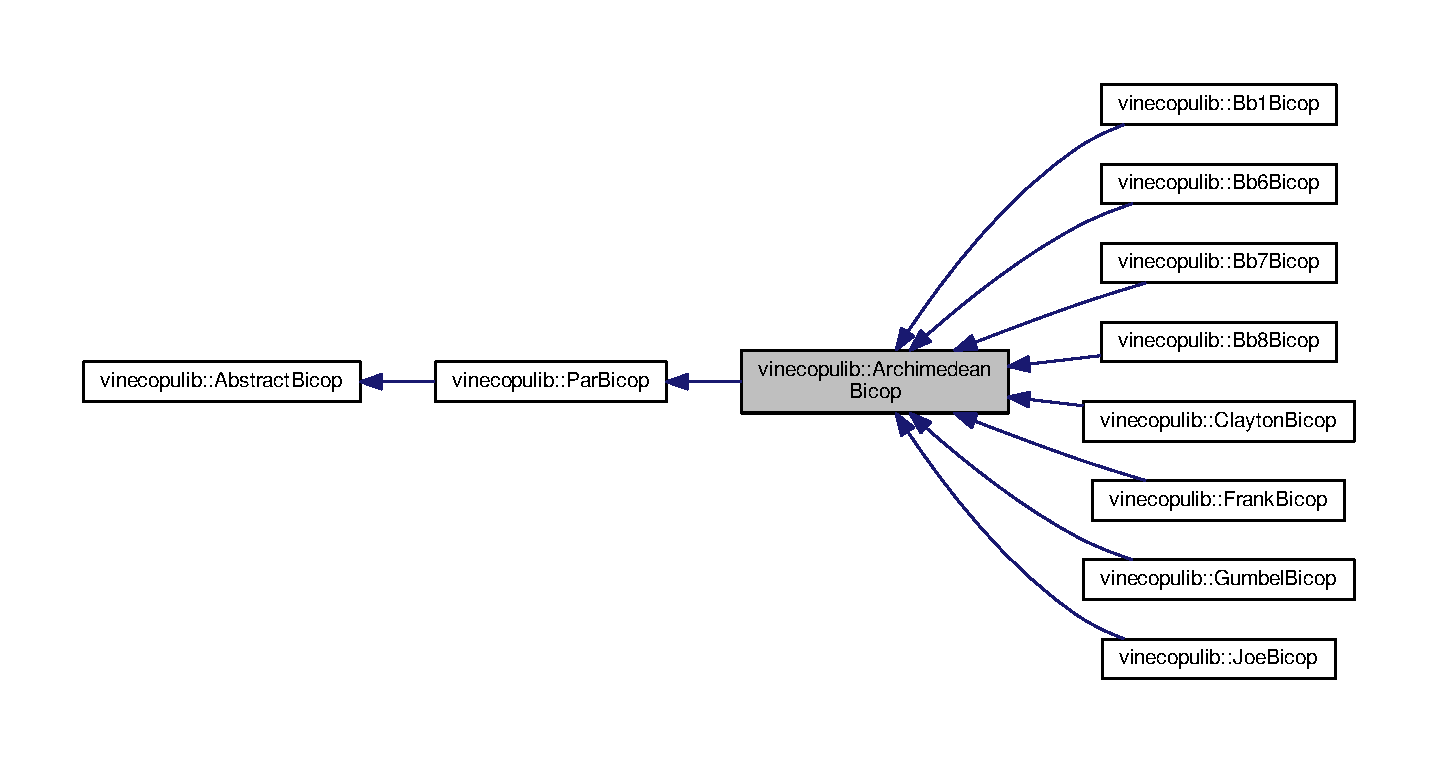
\includegraphics[width=350pt]{classvinecopulib_1_1_archimedean_bicop__inherit__graph}
\end{center}
\end{figure}


Collaboration diagram for vinecopulib\+:\+:Archimedean\+Bicop\+:
\nopagebreak
\begin{figure}[H]
\begin{center}
\leavevmode
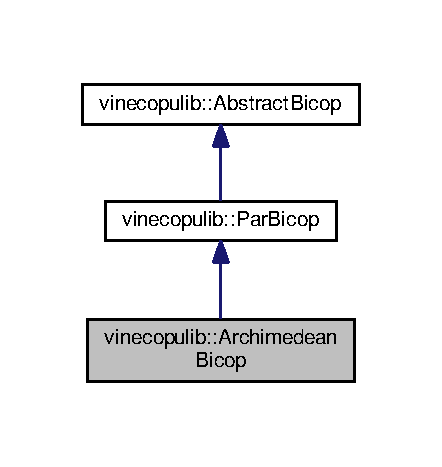
\includegraphics[width=213pt]{classvinecopulib_1_1_archimedean_bicop__coll__graph}
\end{center}
\end{figure}
\subsection*{Additional Inherited Members}


\subsection{Detailed Description}
An abstract class for Archimedean copula families. 

This class is used in the implementation underlying the \hyperlink{classvinecopulib_1_1_bicop}{Bicop} class. Users should not use \hyperlink{classvinecopulib_1_1_abstract_bicop}{Abstract\+Bicop} or derived classes directly, but always work with the \hyperlink{classvinecopulib_1_1_bicop}{Bicop} interface.

Joe, Harry. Dependence modeling with copulas. C\+RC Press, 2014. 

The documentation for this class was generated from the following files\+:\begin{DoxyCompactItemize}
\item 
/home/n5/dev/cpp/vinecopulib/include/bicop/archimedean.\+hpp\item 
/home/n5/dev/cpp/vinecopulib/src/bicop/archimedean.\+cpp\end{DoxyCompactItemize}

\hypertarget{classvinecopulib_1_1_bb1_bicop}{}\section{vinecopulib\+:\+:Bb1\+Bicop Class Reference}
\label{classvinecopulib_1_1_bb1_bicop}\index{vinecopulib\+::\+Bb1\+Bicop@{vinecopulib\+::\+Bb1\+Bicop}}


The B\+B1 copula.  




{\ttfamily \#include $<$bb1.\+hpp$>$}



Inheritance diagram for vinecopulib\+:\+:Bb1\+Bicop\+:
\nopagebreak
\begin{figure}[H]
\begin{center}
\leavevmode
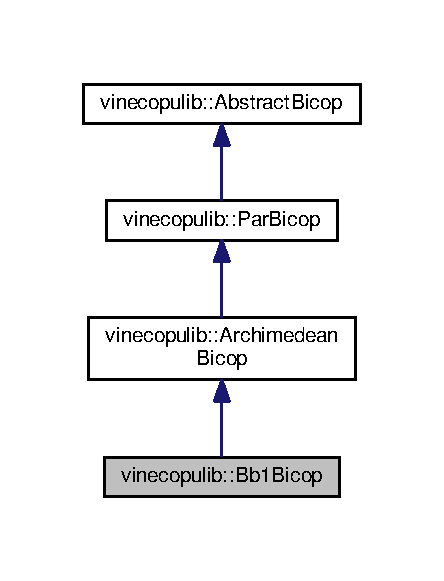
\includegraphics[width=213pt]{classvinecopulib_1_1_bb1_bicop__inherit__graph}
\end{center}
\end{figure}


Collaboration diagram for vinecopulib\+:\+:Bb1\+Bicop\+:
\nopagebreak
\begin{figure}[H]
\begin{center}
\leavevmode
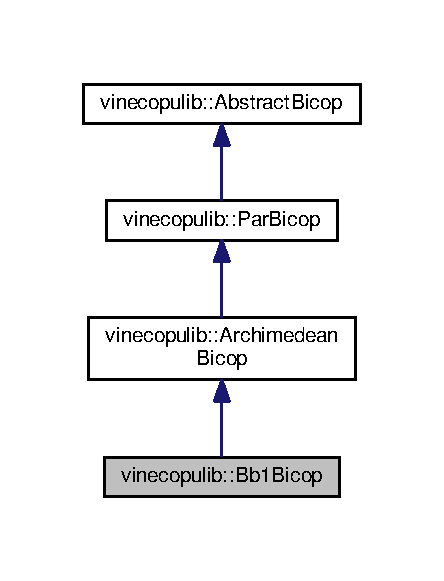
\includegraphics[width=213pt]{classvinecopulib_1_1_bb1_bicop__coll__graph}
\end{center}
\end{figure}
\subsection*{Additional Inherited Members}


\subsection{Detailed Description}
The B\+B1 copula. 

This class is used in the implementation underlying the \hyperlink{classvinecopulib_1_1_bicop}{Bicop} class. Users should not use \hyperlink{classvinecopulib_1_1_abstract_bicop}{Abstract\+Bicop} or derived classes directly, but always work with the \hyperlink{classvinecopulib_1_1_bicop}{Bicop} interface.

Joe, Harry. Dependence modeling with copulas. C\+RC Press, 2014. 

The documentation for this class was generated from the following files\+:\begin{DoxyCompactItemize}
\item 
/home/n5/dev/cpp/vinecopulib/include/bicop/bb1.\+hpp\item 
/home/n5/dev/cpp/vinecopulib/src/bicop/bb1.\+cpp\end{DoxyCompactItemize}

\hypertarget{classvinecopulib_1_1_bb6_bicop}{\section{vinecopulib\+:\+:Bb6\+Bicop Class Reference}
\label{classvinecopulib_1_1_bb6_bicop}\index{vinecopulib\+::\+Bb6\+Bicop@{vinecopulib\+::\+Bb6\+Bicop}}
}


The B\+B6 copula.  




{\ttfamily \#include $<$bb6.\+hpp$>$}



Inheritance diagram for vinecopulib\+:\+:Bb6\+Bicop\+:\nopagebreak
\begin{figure}[H]
\begin{center}
\leavevmode
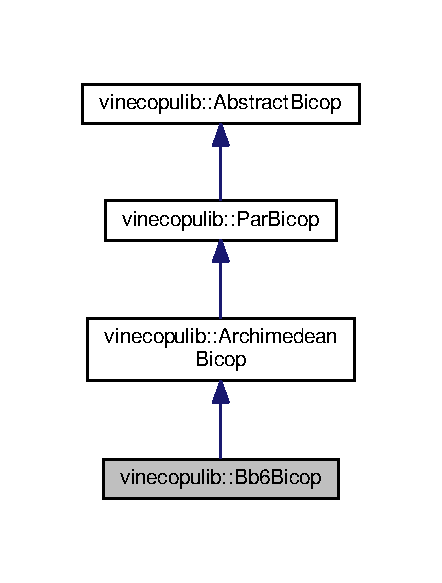
\includegraphics[width=212pt]{classvinecopulib_1_1_bb6_bicop__inherit__graph}
\end{center}
\end{figure}


Collaboration diagram for vinecopulib\+:\+:Bb6\+Bicop\+:\nopagebreak
\begin{figure}[H]
\begin{center}
\leavevmode
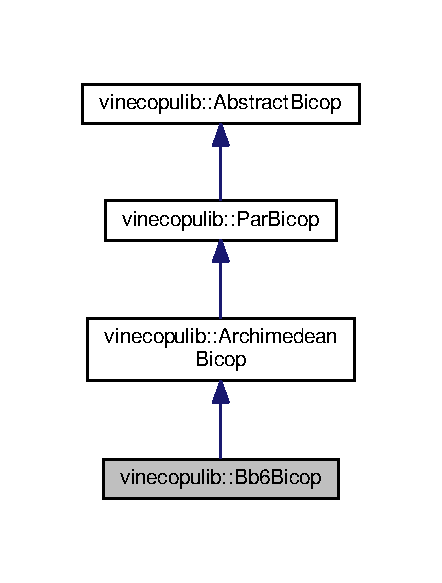
\includegraphics[width=212pt]{classvinecopulib_1_1_bb6_bicop__coll__graph}
\end{center}
\end{figure}
\subsection*{Additional Inherited Members}


\subsection{Detailed Description}
The B\+B6 copula. 

This class is used in the implementation underlying the \hyperlink{classvinecopulib_1_1_bicop}{Bicop} class. Users should not use \hyperlink{classvinecopulib_1_1_abstract_bicop}{Abstract\+Bicop} or derived classes directly, but always work with the \hyperlink{classvinecopulib_1_1_bicop}{Bicop} interface.

Joe, Harry. Dependence modeling with copulas. C\+R\+C Press, 2014. 

The documentation for this class was generated from the following files\+:\begin{DoxyCompactItemize}
\item 
vinecopulib/include/vinecopulib/bicop/bb6.\+hpp\item 
vinecopulib/src/bicop/bb6.\+cpp\end{DoxyCompactItemize}

\hypertarget{classvinecopulib_1_1_bb7_bicop}{}\section{vinecopulib\+:\+:Bb7\+Bicop Class Reference}
\label{classvinecopulib_1_1_bb7_bicop}\index{vinecopulib\+::\+Bb7\+Bicop@{vinecopulib\+::\+Bb7\+Bicop}}


The B\+B7 copula.  




{\ttfamily \#include $<$bb7.\+hpp$>$}



Inheritance diagram for vinecopulib\+:\+:Bb7\+Bicop\+:
\nopagebreak
\begin{figure}[H]
\begin{center}
\leavevmode
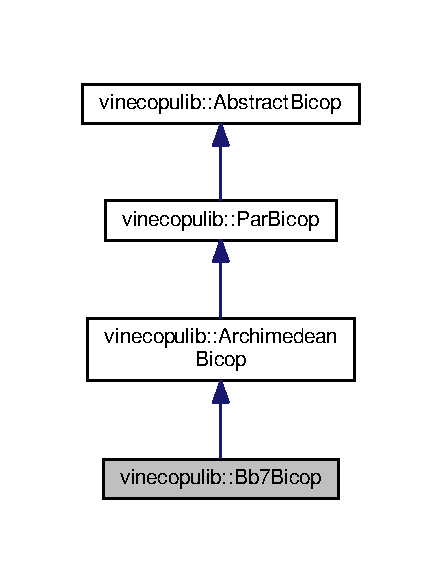
\includegraphics[width=213pt]{classvinecopulib_1_1_bb7_bicop__inherit__graph}
\end{center}
\end{figure}


Collaboration diagram for vinecopulib\+:\+:Bb7\+Bicop\+:
\nopagebreak
\begin{figure}[H]
\begin{center}
\leavevmode
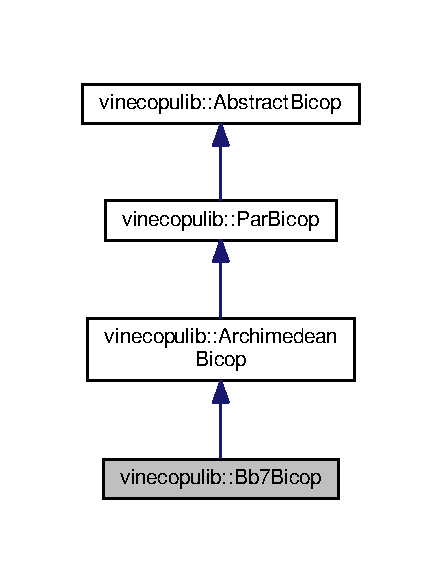
\includegraphics[width=213pt]{classvinecopulib_1_1_bb7_bicop__coll__graph}
\end{center}
\end{figure}
\subsection*{Additional Inherited Members}


\subsection{Detailed Description}
The B\+B7 copula. 

This class is used in the implementation underlying the \hyperlink{classvinecopulib_1_1_bicop}{Bicop} class. Users should not use \hyperlink{classvinecopulib_1_1_abstract_bicop}{Abstract\+Bicop} or derived classes directly, but always work with the \hyperlink{classvinecopulib_1_1_bicop}{Bicop} interface.

Joe, Harry. Dependence modeling with copulas. C\+RC Press, 2014. 

The documentation for this class was generated from the following files\+:\begin{DoxyCompactItemize}
\item 
/home/n5/dev/cpp/vinecopulib/include/bicop/bb7.\+hpp\item 
/home/n5/dev/cpp/vinecopulib/src/bicop/bb7.\+cpp\end{DoxyCompactItemize}

\hypertarget{classvinecopulib_1_1_bb8_bicop}{}\section{vinecopulib\+:\+:Bb8\+Bicop Class Reference}
\label{classvinecopulib_1_1_bb8_bicop}\index{vinecopulib\+::\+Bb8\+Bicop@{vinecopulib\+::\+Bb8\+Bicop}}


Inheritance diagram for vinecopulib\+:\+:Bb8\+Bicop\+:\nopagebreak
\begin{figure}[H]
\begin{center}
\leavevmode
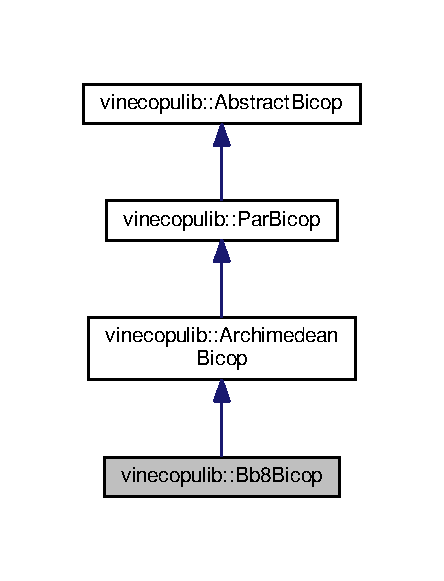
\includegraphics[width=208pt]{classvinecopulib_1_1_bb8_bicop__inherit__graph}
\end{center}
\end{figure}


Collaboration diagram for vinecopulib\+:\+:Bb8\+Bicop\+:\nopagebreak
\begin{figure}[H]
\begin{center}
\leavevmode
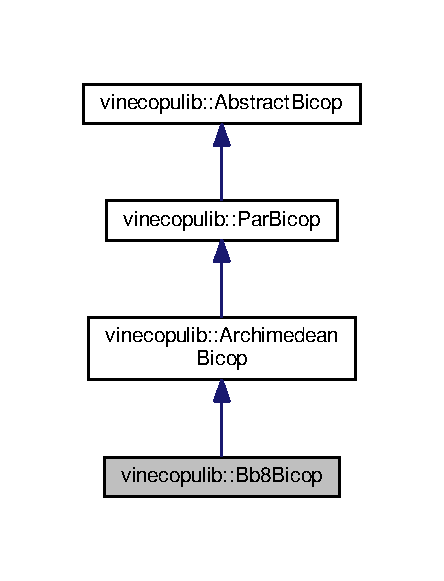
\includegraphics[width=208pt]{classvinecopulib_1_1_bb8_bicop__coll__graph}
\end{center}
\end{figure}
\subsection*{Additional Inherited Members}


The documentation for this class was generated from the following files\+:\begin{DoxyCompactItemize}
\item 
/home/n5/dev/cpp/vinecopulib/include/bicop\+\_\+bb8.\+hpp\item 
/home/n5/dev/cpp/vinecopulib/src/bicop\+\_\+bb8.\+cpp\end{DoxyCompactItemize}

\hypertarget{classvinecopulib_1_1_bicop}{\section{vinecopulib\+:\+:Bicop Class Reference}
\label{classvinecopulib_1_1_bicop}\index{vinecopulib\+::\+Bicop@{vinecopulib\+::\+Bicop}}
}


A class for bivariate copula models.  




{\ttfamily \#include $<$class.\+hpp$>$}

\subsection*{Public Member Functions}
\begin{DoxyCompactItemize}
\item 
\hypertarget{classvinecopulib_1_1_bicop_acfa522fb0bea4aca8fade87c18bcf921}{\hyperlink{classvinecopulib_1_1_bicop_acfa522fb0bea4aca8fade87c18bcf921}{Bicop} ()}\label{classvinecopulib_1_1_bicop_acfa522fb0bea4aca8fade87c18bcf921}

\begin{DoxyCompactList}\small\item\em creates the independence copula. \end{DoxyCompactList}\item 
\hyperlink{classvinecopulib_1_1_bicop_ab27f789e001e30f2fed7f9ecefdeffb0}{Bicop} (\hyperlink{namespacevinecopulib_a42e95cc06d33896199caab0c11ad44f3}{Bicop\+Family} family, int rotation=0, const Eigen\+::\+Matrix\+Xd \&parameters=Eigen\+::\+Matrix\+Xd())
\item 
\hyperlink{classvinecopulib_1_1_bicop_afc8b465d9e02a3df1c25f7c1e7ac9240}{Bicop} (Eigen\+::\+Matrix$<$ double, Eigen\+::\+Dynamic, 2 $>$ data, \hyperlink{classvinecopulib_1_1_fit_controls_bicop}{Fit\+Controls\+Bicop} controls=\hyperlink{classvinecopulib_1_1_fit_controls_bicop}{Fit\+Controls\+Bicop}())
\item 
Eigen\+::\+Vector\+Xd \hyperlink{classvinecopulib_1_1_bicop_a83dc7214e4bb1bfe59285ca05407d646}{pdf} (const Eigen\+::\+Matrix$<$ double, Eigen\+::\+Dynamic, 2 $>$ \&u)
\item 
Eigen\+::\+Vector\+Xd \hyperlink{classvinecopulib_1_1_bicop_a153d7e766388066eda14577c5a6332cc}{cdf} (const Eigen\+::\+Matrix$<$ double, Eigen\+::\+Dynamic, 2 $>$ \&u)
\item 
Eigen\+::\+Vector\+Xd \hyperlink{classvinecopulib_1_1_bicop_a130fda62cd61c7acdef5db75fffdd89e}{hfunc1} (const Eigen\+::\+Matrix$<$ double, Eigen\+::\+Dynamic, 2 $>$ \&u)
\item 
Eigen\+::\+Vector\+Xd \hyperlink{classvinecopulib_1_1_bicop_a4c9b50f99797ec374f5057cc54db2bd8}{hfunc2} (const Eigen\+::\+Matrix$<$ double, Eigen\+::\+Dynamic, 2 $>$ \&u)
\item 
Eigen\+::\+Vector\+Xd \hyperlink{classvinecopulib_1_1_bicop_a3cc8b161ec6efdb3b34d2efa9185bf44}{hinv1} (const Eigen\+::\+Matrix$<$ double, Eigen\+::\+Dynamic, 2 $>$ \&u)
\item 
Eigen\+::\+Vector\+Xd \hyperlink{classvinecopulib_1_1_bicop_a3e33ec227b6b7182e327399201cad382}{hinv2} (const Eigen\+::\+Matrix$<$ double, Eigen\+::\+Dynamic, 2 $>$ \&u)
\item 
Eigen\+::\+Matrix$<$ double, \\*
Eigen\+::\+Dynamic, 2 $>$ \hyperlink{classvinecopulib_1_1_bicop_aeb87bea4283dacfa5e609356c020f85d}{simulate} (const int \&n)
\item 
void \hyperlink{classvinecopulib_1_1_bicop_a2d509a8b404a73ef17f04a0678e90a71}{fit} (const Eigen\+::\+Matrix$<$ double, Eigen\+::\+Dynamic, 2 $>$ \&data, \hyperlink{classvinecopulib_1_1_fit_controls_bicop}{Fit\+Controls\+Bicop} controls=\hyperlink{classvinecopulib_1_1_fit_controls_bicop}{Fit\+Controls\+Bicop}())
\item 
void \hyperlink{classvinecopulib_1_1_bicop_af20af5c3ba6565628987b4784e9ac348}{select} (Eigen\+::\+Matrix$<$ double, Eigen\+::\+Dynamic, 2 $>$ data, \hyperlink{classvinecopulib_1_1_fit_controls_bicop}{Fit\+Controls\+Bicop} controls=\hyperlink{classvinecopulib_1_1_fit_controls_bicop}{Fit\+Controls\+Bicop}())
\item 
double \hyperlink{classvinecopulib_1_1_bicop_ae8bcc0c3265cc86565333a0cfd3d619d}{loglik} (const Eigen\+::\+Matrix$<$ double, Eigen\+::\+Dynamic, 2 $>$ \&u)
\item 
double \hyperlink{classvinecopulib_1_1_bicop_a9287fec95519fea64a2ae80f5888c709}{aic} (const Eigen\+::\+Matrix$<$ double, Eigen\+::\+Dynamic, 2 $>$ \&u)
\item 
double \hyperlink{classvinecopulib_1_1_bicop_ac1f480d13b3464260c2dd6aa88b2e130}{bic} (const Eigen\+::\+Matrix$<$ double, Eigen\+::\+Dynamic, 2 $>$ \&u)
\item 
double \hyperlink{classvinecopulib_1_1_bicop_a9f3b3b83c54a9e1d809fdee058f3eb11}{calculate\+\_\+npars} ()
\item 
double \hyperlink{classvinecopulib_1_1_bicop_aa25436353dee76e4368fb941a7efa257}{parameters\+\_\+to\+\_\+tau} (const Eigen\+::\+Vector\+Xd \&parameters)
\item 
Eigen\+::\+Matrix\+Xd \hyperlink{classvinecopulib_1_1_bicop_a5809ddc9884f6fb66fe53289be348913}{tau\+\_\+to\+\_\+parameters} (const double \&tau)
\end{DoxyCompactItemize}
\begin{Indent}{\bf Getters and setters}\par
\begin{DoxyCompactItemize}
\item 
\hypertarget{classvinecopulib_1_1_bicop_a68ab3556ee3bb3d02814fd978573bf3b}{\hyperlink{namespacevinecopulib_a42e95cc06d33896199caab0c11ad44f3}{Bicop\+Family} {\bfseries get\+\_\+family} () const }\label{classvinecopulib_1_1_bicop_a68ab3556ee3bb3d02814fd978573bf3b}

\item 
\hypertarget{classvinecopulib_1_1_bicop_a4d4fbc0fdca17564c23f4814d5d2fbe7}{std\+::string {\bfseries get\+\_\+family\+\_\+name} () const }\label{classvinecopulib_1_1_bicop_a4d4fbc0fdca17564c23f4814d5d2fbe7}

\item 
\hypertarget{classvinecopulib_1_1_bicop_ab8e52577a50fbfc57277f9240d8eac03}{int {\bfseries get\+\_\+rotation} () const }\label{classvinecopulib_1_1_bicop_ab8e52577a50fbfc57277f9240d8eac03}

\item 
\hypertarget{classvinecopulib_1_1_bicop_a93ab0dd89826e50b209ea3760f251f2f}{Eigen\+::\+Matrix\+Xd {\bfseries get\+\_\+parameters} () const }\label{classvinecopulib_1_1_bicop_a93ab0dd89826e50b209ea3760f251f2f}

\item 
void \hyperlink{classvinecopulib_1_1_bicop_a4e359624560a089273b25dc74879bd16}{set\+\_\+rotation} (int rotation)
\item 
void \hyperlink{classvinecopulib_1_1_bicop_ac8d1d4266b0fd7e2f971d0149f881ef9}{set\+\_\+parameters} (const Eigen\+::\+Matrix\+Xd \&parameters)
\end{DoxyCompactItemize}
\end{Indent}
\begin{Indent}{\bf Utilities}\par
{\em adjust's the copula model to a change in the variable order. }\begin{DoxyCompactItemize}
\item 
\hypertarget{classvinecopulib_1_1_bicop_a94b889d56f478dbeb156be4e31af5de5}{std\+::string \hyperlink{classvinecopulib_1_1_bicop_a94b889d56f478dbeb156be4e31af5de5}{str} ()}\label{classvinecopulib_1_1_bicop_a94b889d56f478dbeb156be4e31af5de5}

\begin{DoxyCompactList}\small\item\em summarizes the model into a string (can be used for printing). \end{DoxyCompactList}\item 
\hypertarget{classvinecopulib_1_1_bicop_a59b7087b3857350df25ff684ab96f377}{void {\bfseries flip} ()}\label{classvinecopulib_1_1_bicop_a59b7087b3857350df25ff684ab96f377}

\end{DoxyCompactItemize}
\end{Indent}


\subsection{Detailed Description}
A class for bivariate copula models. 

The copula model is fully characterized by the family, rotation, and parameters. 

\subsection{Constructor \& Destructor Documentation}
\hypertarget{classvinecopulib_1_1_bicop_ab27f789e001e30f2fed7f9ecefdeffb0}{\index{vinecopulib\+::\+Bicop@{vinecopulib\+::\+Bicop}!Bicop@{Bicop}}
\index{Bicop@{Bicop}!vinecopulib\+::\+Bicop@{vinecopulib\+::\+Bicop}}
\subsubsection[{Bicop}]{\setlength{\rightskip}{0pt plus 5cm}vinecopulib\+::\+Bicop\+::\+Bicop (
\begin{DoxyParamCaption}
\item[{{\bf Bicop\+Family}}]{family, }
\item[{int}]{rotation = {\ttfamily 0}, }
\item[{const Eigen\+::\+Matrix\+Xd \&}]{parameters = {\ttfamily Eigen\+:\+:MatrixXd()}}
\end{DoxyParamCaption}
)}}\label{classvinecopulib_1_1_bicop_ab27f789e001e30f2fed7f9ecefdeffb0}
creates a specific bivariate copula model. 
\begin{DoxyParams}{Parameters}
{\em family} & the copula family. \\
\hline
{\em rotation} & the rotation of the copula; one of 0, 90, 180, or 270 (for Independence, Gaussian, Student, Frank, and nonparametric families, only 0 is allowed). \\
\hline
{\em parameters} & the copula parameters. \\
\hline
\end{DoxyParams}
\hypertarget{classvinecopulib_1_1_bicop_afc8b465d9e02a3df1c25f7c1e7ac9240}{\index{vinecopulib\+::\+Bicop@{vinecopulib\+::\+Bicop}!Bicop@{Bicop}}
\index{Bicop@{Bicop}!vinecopulib\+::\+Bicop@{vinecopulib\+::\+Bicop}}
\subsubsection[{Bicop}]{\setlength{\rightskip}{0pt plus 5cm}vinecopulib\+::\+Bicop\+::\+Bicop (
\begin{DoxyParamCaption}
\item[{Eigen\+::\+Matrix$<$ double, Eigen\+::\+Dynamic, 2 $>$}]{data, }
\item[{{\bf Fit\+Controls\+Bicop}}]{controls = {\ttfamily {\bf Fit\+Controls\+Bicop}()}}
\end{DoxyParamCaption}
)}}\label{classvinecopulib_1_1_bicop_afc8b465d9e02a3df1c25f7c1e7ac9240}
equivalent to {\ttfamily \hyperlink{classvinecopulib_1_1_bicop}{Bicop} cop; cop.\+select(data, controls)}. 
\begin{DoxyParams}{Parameters}
{\em data} & see \hyperlink{classvinecopulib_1_1_bicop_af20af5c3ba6565628987b4784e9ac348}{select()}. \\
\hline
{\em controls} & see \hyperlink{classvinecopulib_1_1_bicop_af20af5c3ba6565628987b4784e9ac348}{select()}. \\
\hline
\end{DoxyParams}


\subsection{Member Function Documentation}
\hypertarget{classvinecopulib_1_1_bicop_a9287fec95519fea64a2ae80f5888c709}{\index{vinecopulib\+::\+Bicop@{vinecopulib\+::\+Bicop}!aic@{aic}}
\index{aic@{aic}!vinecopulib\+::\+Bicop@{vinecopulib\+::\+Bicop}}
\subsubsection[{aic}]{\setlength{\rightskip}{0pt plus 5cm}double vinecopulib\+::\+Bicop\+::aic (
\begin{DoxyParamCaption}
\item[{const Eigen\+::\+Matrix$<$ double, Eigen\+::\+Dynamic, 2 $>$ \&}]{u}
\end{DoxyParamCaption}
)}}\label{classvinecopulib_1_1_bicop_a9287fec95519fea64a2ae80f5888c709}
calculates the Akaike information criterion (A\+I\+C).

The A\+I\+C is defined as \[ \mathrm{AIC} = -2\, \mathrm{loglik} + 2 p, \] where $ \mathrm{loglik} $ is the log-\/liklihood and $ p $ is the (effective) number of parameters of the model, see \hyperlink{classvinecopulib_1_1_bicop_ae8bcc0c3265cc86565333a0cfd3d619d}{loglik()} and \hyperlink{classvinecopulib_1_1_bicop_a9f3b3b83c54a9e1d809fdee058f3eb11}{calculate\+\_\+npars()}. The A\+I\+C is a consistent model selection criterion for nonparametric models.


\begin{DoxyParams}{Parameters}
{\em u} & $n \times 2$ matrix of observations. \\
\hline
\end{DoxyParams}
\hypertarget{classvinecopulib_1_1_bicop_ac1f480d13b3464260c2dd6aa88b2e130}{\index{vinecopulib\+::\+Bicop@{vinecopulib\+::\+Bicop}!bic@{bic}}
\index{bic@{bic}!vinecopulib\+::\+Bicop@{vinecopulib\+::\+Bicop}}
\subsubsection[{bic}]{\setlength{\rightskip}{0pt plus 5cm}double vinecopulib\+::\+Bicop\+::bic (
\begin{DoxyParamCaption}
\item[{const Eigen\+::\+Matrix$<$ double, Eigen\+::\+Dynamic, 2 $>$ \&}]{u}
\end{DoxyParamCaption}
)}}\label{classvinecopulib_1_1_bicop_ac1f480d13b3464260c2dd6aa88b2e130}
calculates the Bayesian information criterion (B\+I\+C).

The B\+I\+C is defined as \[ \mathrm{BIC} = -2\, \mathrm{loglik} + \ln(n) p, \] where $ \mathrm{loglik} $ is the log-\/liklihood and $ p $ is the (effective) number of parameters of the model, see \hyperlink{classvinecopulib_1_1_bicop_ae8bcc0c3265cc86565333a0cfd3d619d}{loglik()} and \hyperlink{classvinecopulib_1_1_bicop_a9f3b3b83c54a9e1d809fdee058f3eb11}{calculate\+\_\+npars()}. The B\+I\+C is a consistent model selection criterion for nonparametric models.


\begin{DoxyParams}{Parameters}
{\em u} & $n \times 2$ matrix of observations. \\
\hline
\end{DoxyParams}
\hypertarget{classvinecopulib_1_1_bicop_a9f3b3b83c54a9e1d809fdee058f3eb11}{\index{vinecopulib\+::\+Bicop@{vinecopulib\+::\+Bicop}!calculate\+\_\+npars@{calculate\+\_\+npars}}
\index{calculate\+\_\+npars@{calculate\+\_\+npars}!vinecopulib\+::\+Bicop@{vinecopulib\+::\+Bicop}}
\subsubsection[{calculate\+\_\+npars}]{\setlength{\rightskip}{0pt plus 5cm}double vinecopulib\+::\+Bicop\+::calculate\+\_\+npars (
\begin{DoxyParamCaption}
{}
\end{DoxyParamCaption}
)}}\label{classvinecopulib_1_1_bicop_a9f3b3b83c54a9e1d809fdee058f3eb11}
calculates the effective number of parameters.

Returns the actual number of parameters for parameteric families. For nonparametric families, there is a conceptually similar definition in the sense that it can be used in the calculation of fit statistics. \hypertarget{classvinecopulib_1_1_bicop_a153d7e766388066eda14577c5a6332cc}{\index{vinecopulib\+::\+Bicop@{vinecopulib\+::\+Bicop}!cdf@{cdf}}
\index{cdf@{cdf}!vinecopulib\+::\+Bicop@{vinecopulib\+::\+Bicop}}
\subsubsection[{cdf}]{\setlength{\rightskip}{0pt plus 5cm}Eigen\+::\+Vector\+Xd vinecopulib\+::\+Bicop\+::cdf (
\begin{DoxyParamCaption}
\item[{const Eigen\+::\+Matrix$<$ double, Eigen\+::\+Dynamic, 2 $>$ \&}]{u}
\end{DoxyParamCaption}
)}}\label{classvinecopulib_1_1_bicop_a153d7e766388066eda14577c5a6332cc}
evaluates the copula distribution.


\begin{DoxyParams}{Parameters}
{\em u} & $n \times 2$ matrix of evaluation points. \\
\hline
\end{DoxyParams}
\begin{DoxyReturn}{Returns}
The copula distribution evaluated at {\ttfamily u}. 
\end{DoxyReturn}
\hypertarget{classvinecopulib_1_1_bicop_a2d509a8b404a73ef17f04a0678e90a71}{\index{vinecopulib\+::\+Bicop@{vinecopulib\+::\+Bicop}!fit@{fit}}
\index{fit@{fit}!vinecopulib\+::\+Bicop@{vinecopulib\+::\+Bicop}}
\subsubsection[{fit}]{\setlength{\rightskip}{0pt plus 5cm}void vinecopulib\+::\+Bicop\+::fit (
\begin{DoxyParamCaption}
\item[{const Eigen\+::\+Matrix$<$ double, Eigen\+::\+Dynamic, 2 $>$ \&}]{data, }
\item[{{\bf Fit\+Controls\+Bicop}}]{controls = {\ttfamily {\bf Fit\+Controls\+Bicop}()}}
\end{DoxyParamCaption}
)}}\label{classvinecopulib_1_1_bicop_a2d509a8b404a73ef17f04a0678e90a71}
fits a bivariate copula (with fixed family) to data.

For parametric models, two different methods are available. {\ttfamily \char`\"{}mle\char`\"{}} fits the parameters by maximum-\/likelihood. {\ttfamily \char`\"{}itau\char`\"{}} uses inversion of Kendall's $ \tau $, but is only available for one-\/parameter families and the Student t copula. For the latter, there is a one-\/to-\/one transformation for the first parameter, the second is found by profile likelihood optimization (with accuracy of at least 0.\+5). Nonparametric families have specialized methods, no specification is required.


\begin{DoxyParams}{Parameters}
{\em data} & an $ n \times 2 $ matrix of observations contained in $(0, 1)^2 $. \\
\hline
{\em controls} & the controls (see \hyperlink{classvinecopulib_1_1_fit_controls_bicop}{Fit\+Controls\+Bicop}). \\
\hline
\end{DoxyParams}
\hypertarget{classvinecopulib_1_1_bicop_a130fda62cd61c7acdef5db75fffdd89e}{\index{vinecopulib\+::\+Bicop@{vinecopulib\+::\+Bicop}!hfunc1@{hfunc1}}
\index{hfunc1@{hfunc1}!vinecopulib\+::\+Bicop@{vinecopulib\+::\+Bicop}}
\subsubsection[{hfunc1}]{\setlength{\rightskip}{0pt plus 5cm}Eigen\+::\+Vector\+Xd vinecopulib\+::\+Bicop\+::hfunc1 (
\begin{DoxyParamCaption}
\item[{const Eigen\+::\+Matrix$<$ double, Eigen\+::\+Dynamic, 2 $>$ \&}]{u}
\end{DoxyParamCaption}
)}}\label{classvinecopulib_1_1_bicop_a130fda62cd61c7acdef5db75fffdd89e}
calculates the first h-\/function, i.\+e., $ h_1(u_1, u_2) = \int_0^{u_2} c(u_1, s) $. 
\begin{DoxyParams}{Parameters}
{\em u} & $m \times 2$ matrix of evaluation points. \\
\hline
\end{DoxyParams}
\hypertarget{classvinecopulib_1_1_bicop_a4c9b50f99797ec374f5057cc54db2bd8}{\index{vinecopulib\+::\+Bicop@{vinecopulib\+::\+Bicop}!hfunc2@{hfunc2}}
\index{hfunc2@{hfunc2}!vinecopulib\+::\+Bicop@{vinecopulib\+::\+Bicop}}
\subsubsection[{hfunc2}]{\setlength{\rightskip}{0pt plus 5cm}Eigen\+::\+Vector\+Xd vinecopulib\+::\+Bicop\+::hfunc2 (
\begin{DoxyParamCaption}
\item[{const Eigen\+::\+Matrix$<$ double, Eigen\+::\+Dynamic, 2 $>$ \&}]{u}
\end{DoxyParamCaption}
)}}\label{classvinecopulib_1_1_bicop_a4c9b50f99797ec374f5057cc54db2bd8}
calculates the second h-\/function, i.\+e., $ h_2(u_1, u_2) = \int_0^{u_1} c(s, u_2) $. 
\begin{DoxyParams}{Parameters}
{\em u} & $m \times 2$ matrix of evaluation points. \\
\hline
\end{DoxyParams}
\hypertarget{classvinecopulib_1_1_bicop_a3cc8b161ec6efdb3b34d2efa9185bf44}{\index{vinecopulib\+::\+Bicop@{vinecopulib\+::\+Bicop}!hinv1@{hinv1}}
\index{hinv1@{hinv1}!vinecopulib\+::\+Bicop@{vinecopulib\+::\+Bicop}}
\subsubsection[{hinv1}]{\setlength{\rightskip}{0pt plus 5cm}Eigen\+::\+Vector\+Xd vinecopulib\+::\+Bicop\+::hinv1 (
\begin{DoxyParamCaption}
\item[{const Eigen\+::\+Matrix$<$ double, Eigen\+::\+Dynamic, 2 $>$ \&}]{u}
\end{DoxyParamCaption}
)}}\label{classvinecopulib_1_1_bicop_a3cc8b161ec6efdb3b34d2efa9185bf44}
calculates the inverse of $ h_1 f$ (see \hyperlink{classvinecopulib_1_1_bicop_a130fda62cd61c7acdef5db75fffdd89e}{hfunc1()}) w.\+r.\+t. the second argument. 
\begin{DoxyParams}{Parameters}
{\em u} & $m \times 2$ matrix of evaluation points. \\
\hline
\end{DoxyParams}
\hypertarget{classvinecopulib_1_1_bicop_a3e33ec227b6b7182e327399201cad382}{\index{vinecopulib\+::\+Bicop@{vinecopulib\+::\+Bicop}!hinv2@{hinv2}}
\index{hinv2@{hinv2}!vinecopulib\+::\+Bicop@{vinecopulib\+::\+Bicop}}
\subsubsection[{hinv2}]{\setlength{\rightskip}{0pt plus 5cm}Eigen\+::\+Vector\+Xd vinecopulib\+::\+Bicop\+::hinv2 (
\begin{DoxyParamCaption}
\item[{const Eigen\+::\+Matrix$<$ double, Eigen\+::\+Dynamic, 2 $>$ \&}]{u}
\end{DoxyParamCaption}
)}}\label{classvinecopulib_1_1_bicop_a3e33ec227b6b7182e327399201cad382}
calculates the inverse of $ h_2 f$ (see \hyperlink{classvinecopulib_1_1_bicop_a4c9b50f99797ec374f5057cc54db2bd8}{hfunc2()}) w.\+r.\+t. the first argument. 
\begin{DoxyParams}{Parameters}
{\em u} & $m \times 2$ matrix of evaluation points. \\
\hline
\end{DoxyParams}
\hypertarget{classvinecopulib_1_1_bicop_ae8bcc0c3265cc86565333a0cfd3d619d}{\index{vinecopulib\+::\+Bicop@{vinecopulib\+::\+Bicop}!loglik@{loglik}}
\index{loglik@{loglik}!vinecopulib\+::\+Bicop@{vinecopulib\+::\+Bicop}}
\subsubsection[{loglik}]{\setlength{\rightskip}{0pt plus 5cm}double vinecopulib\+::\+Bicop\+::loglik (
\begin{DoxyParamCaption}
\item[{const Eigen\+::\+Matrix$<$ double, Eigen\+::\+Dynamic, 2 $>$ \&}]{u}
\end{DoxyParamCaption}
)}}\label{classvinecopulib_1_1_bicop_ae8bcc0c3265cc86565333a0cfd3d619d}
calculates the log-\/likelihood.

The log-\/likelihood is defined as \[ \mathrm{loglik} = \sum_{i = 1}^n \ln c(U_{1, i}, U_{2, i}), \] where $ c $ is the copula density \hyperlink{classvinecopulib_1_1_bicop_a83dc7214e4bb1bfe59285ca05407d646}{pdf()}.


\begin{DoxyParams}{Parameters}
{\em u} & $n \times 2$ matrix of observations. \\
\hline
\end{DoxyParams}
\hypertarget{classvinecopulib_1_1_bicop_aa25436353dee76e4368fb941a7efa257}{\index{vinecopulib\+::\+Bicop@{vinecopulib\+::\+Bicop}!parameters\+\_\+to\+\_\+tau@{parameters\+\_\+to\+\_\+tau}}
\index{parameters\+\_\+to\+\_\+tau@{parameters\+\_\+to\+\_\+tau}!vinecopulib\+::\+Bicop@{vinecopulib\+::\+Bicop}}
\subsubsection[{parameters\+\_\+to\+\_\+tau}]{\setlength{\rightskip}{0pt plus 5cm}double vinecopulib\+::\+Bicop\+::parameters\+\_\+to\+\_\+tau (
\begin{DoxyParamCaption}
\item[{const Eigen\+::\+Vector\+Xd \&}]{parameters}
\end{DoxyParamCaption}
)}}\label{classvinecopulib_1_1_bicop_aa25436353dee76e4368fb941a7efa257}
converts the parameters to the Kendall's $ tau $ for the current family (works for all families but {\ttfamily \hyperlink{namespacevinecopulib_a42e95cc06d33896199caab0c11ad44f3acd36652e61e82e7935de462b329cc8e6}{Bicop\+Family\+::tll0}}).


\begin{DoxyParams}{Parameters}
{\em parameters} & the parameters (must be a valid parametrization of the current family). \\
\hline
\end{DoxyParams}
\hypertarget{classvinecopulib_1_1_bicop_a83dc7214e4bb1bfe59285ca05407d646}{\index{vinecopulib\+::\+Bicop@{vinecopulib\+::\+Bicop}!pdf@{pdf}}
\index{pdf@{pdf}!vinecopulib\+::\+Bicop@{vinecopulib\+::\+Bicop}}
\subsubsection[{pdf}]{\setlength{\rightskip}{0pt plus 5cm}Eigen\+::\+Vector\+Xd vinecopulib\+::\+Bicop\+::pdf (
\begin{DoxyParamCaption}
\item[{const Eigen\+::\+Matrix$<$ double, Eigen\+::\+Dynamic, 2 $>$ \&}]{u}
\end{DoxyParamCaption}
)}}\label{classvinecopulib_1_1_bicop_a83dc7214e4bb1bfe59285ca05407d646}
evaluates the copula density.


\begin{DoxyParams}{Parameters}
{\em u} & $n \times 2$ matrix of evaluation points. \\
\hline
\end{DoxyParams}
\begin{DoxyReturn}{Returns}
The copula density evaluated at {\ttfamily u}. 
\end{DoxyReturn}
\hypertarget{classvinecopulib_1_1_bicop_af20af5c3ba6565628987b4784e9ac348}{\index{vinecopulib\+::\+Bicop@{vinecopulib\+::\+Bicop}!select@{select}}
\index{select@{select}!vinecopulib\+::\+Bicop@{vinecopulib\+::\+Bicop}}
\subsubsection[{select}]{\setlength{\rightskip}{0pt plus 5cm}void vinecopulib\+::\+Bicop\+::select (
\begin{DoxyParamCaption}
\item[{Eigen\+::\+Matrix$<$ double, Eigen\+::\+Dynamic, 2 $>$}]{data, }
\item[{{\bf Fit\+Controls\+Bicop}}]{controls = {\ttfamily {\bf Fit\+Controls\+Bicop}()}}
\end{DoxyParamCaption}
)}}\label{classvinecopulib_1_1_bicop_af20af5c3ba6565628987b4784e9ac348}
selects the best fitting model.

The function calls \hyperlink{classvinecopulib_1_1_bicop_a2d509a8b404a73ef17f04a0678e90a71}{fit()} for all families in {\ttfamily family\+\_\+set}) and selects the best fitting model by either B\+I\+C or A\+I\+C, see \hyperlink{classvinecopulib_1_1_bicop_ac1f480d13b3464260c2dd6aa88b2e130}{bic()} and \hyperlink{classvinecopulib_1_1_bicop_a9287fec95519fea64a2ae80f5888c709}{aic()}.


\begin{DoxyParams}{Parameters}
{\em data} & an $ n \times 2 $ matrix of observations contained in $(0, 1)^2 $. \\
\hline
{\em controls} & the controls (see \hyperlink{classvinecopulib_1_1_fit_controls_bicop}{Fit\+Controls\+Bicop}). \\
\hline
\end{DoxyParams}
\hypertarget{classvinecopulib_1_1_bicop_ac8d1d4266b0fd7e2f971d0149f881ef9}{\index{vinecopulib\+::\+Bicop@{vinecopulib\+::\+Bicop}!set\+\_\+parameters@{set\+\_\+parameters}}
\index{set\+\_\+parameters@{set\+\_\+parameters}!vinecopulib\+::\+Bicop@{vinecopulib\+::\+Bicop}}
\subsubsection[{set\+\_\+parameters}]{\setlength{\rightskip}{0pt plus 5cm}void vinecopulib\+::\+Bicop\+::set\+\_\+parameters (
\begin{DoxyParamCaption}
\item[{const Eigen\+::\+Matrix\+Xd \&}]{parameters}
\end{DoxyParamCaption}
)}}\label{classvinecopulib_1_1_bicop_ac8d1d4266b0fd7e2f971d0149f881ef9}

\begin{DoxyParams}{Parameters}
{\em parameters} & \\
\hline
\end{DoxyParams}
\hypertarget{classvinecopulib_1_1_bicop_a4e359624560a089273b25dc74879bd16}{\index{vinecopulib\+::\+Bicop@{vinecopulib\+::\+Bicop}!set\+\_\+rotation@{set\+\_\+rotation}}
\index{set\+\_\+rotation@{set\+\_\+rotation}!vinecopulib\+::\+Bicop@{vinecopulib\+::\+Bicop}}
\subsubsection[{set\+\_\+rotation}]{\setlength{\rightskip}{0pt plus 5cm}void vinecopulib\+::\+Bicop\+::set\+\_\+rotation (
\begin{DoxyParamCaption}
\item[{int}]{rotation}
\end{DoxyParamCaption}
)}}\label{classvinecopulib_1_1_bicop_a4e359624560a089273b25dc74879bd16}

\begin{DoxyParams}{Parameters}
{\em rotation} & \\
\hline
\end{DoxyParams}
\hypertarget{classvinecopulib_1_1_bicop_aeb87bea4283dacfa5e609356c020f85d}{\index{vinecopulib\+::\+Bicop@{vinecopulib\+::\+Bicop}!simulate@{simulate}}
\index{simulate@{simulate}!vinecopulib\+::\+Bicop@{vinecopulib\+::\+Bicop}}
\subsubsection[{simulate}]{\setlength{\rightskip}{0pt plus 5cm}Eigen\+::\+Matrix$<$ double, Eigen\+::\+Dynamic, 2 $>$ vinecopulib\+::\+Bicop\+::simulate (
\begin{DoxyParamCaption}
\item[{const int \&}]{n}
\end{DoxyParamCaption}
)}}\label{classvinecopulib_1_1_bicop_aeb87bea4283dacfa5e609356c020f85d}
simulates from a bivariate copula.


\begin{DoxyParams}{Parameters}
{\em n} & number of observations. \\
\hline
\end{DoxyParams}
\begin{DoxyReturn}{Returns}
An $ n \times 2 $ matrix of samples from the copula model. 
\end{DoxyReturn}
\hypertarget{classvinecopulib_1_1_bicop_a5809ddc9884f6fb66fe53289be348913}{\index{vinecopulib\+::\+Bicop@{vinecopulib\+::\+Bicop}!tau\+\_\+to\+\_\+parameters@{tau\+\_\+to\+\_\+parameters}}
\index{tau\+\_\+to\+\_\+parameters@{tau\+\_\+to\+\_\+parameters}!vinecopulib\+::\+Bicop@{vinecopulib\+::\+Bicop}}
\subsubsection[{tau\+\_\+to\+\_\+parameters}]{\setlength{\rightskip}{0pt plus 5cm}Eigen\+::\+Matrix\+Xd vinecopulib\+::\+Bicop\+::tau\+\_\+to\+\_\+parameters (
\begin{DoxyParamCaption}
\item[{const double \&}]{tau}
\end{DoxyParamCaption}
)}}\label{classvinecopulib_1_1_bicop_a5809ddc9884f6fb66fe53289be348913}
converts a Kendall's $ \tau $ to the copula parameters of the current family (only works for one-\/parameter families).


\begin{DoxyParams}{Parameters}
{\em tau} & a value in $ (-1, 1) $. \\
\hline
\end{DoxyParams}


The documentation for this class was generated from the following files\+:\begin{DoxyCompactItemize}
\item 
vinecopulib/include/vinecopulib/bicop/class.\+hpp\item 
vinecopulib/src/bicop/class.\+cpp\end{DoxyCompactItemize}

\hypertarget{classvinecopulib_1_1_clayton_bicop}{}\section{vinecopulib\+:\+:Clayton\+Bicop Class Reference}
\label{classvinecopulib_1_1_clayton_bicop}\index{vinecopulib\+::\+Clayton\+Bicop@{vinecopulib\+::\+Clayton\+Bicop}}


Inheritance diagram for vinecopulib\+:\+:Clayton\+Bicop\+:\nopagebreak
\begin{figure}[H]
\begin{center}
\leavevmode
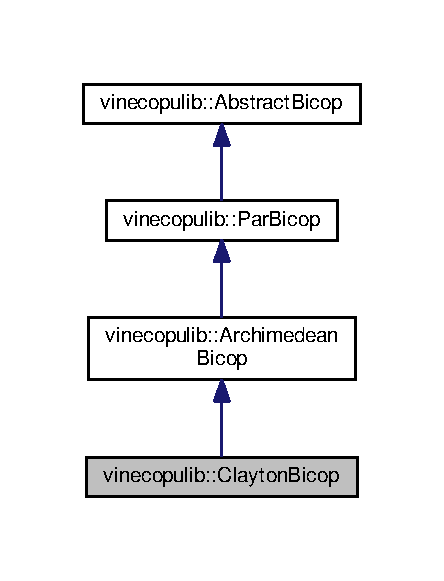
\includegraphics[width=210pt]{classvinecopulib_1_1_clayton_bicop__inherit__graph}
\end{center}
\end{figure}


Collaboration diagram for vinecopulib\+:\+:Clayton\+Bicop\+:\nopagebreak
\begin{figure}[H]
\begin{center}
\leavevmode
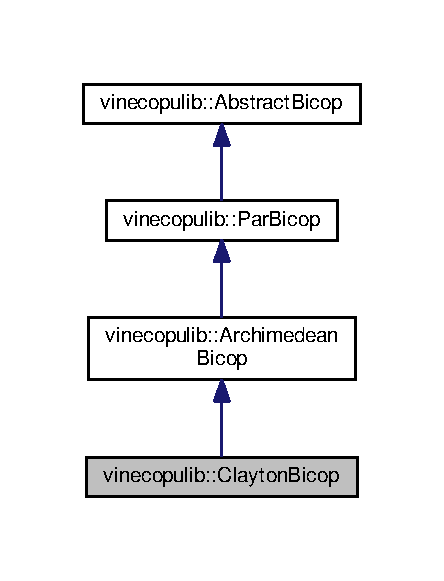
\includegraphics[width=210pt]{classvinecopulib_1_1_clayton_bicop__coll__graph}
\end{center}
\end{figure}
\subsection*{Additional Inherited Members}


The documentation for this class was generated from the following files\+:\begin{DoxyCompactItemize}
\item 
/home/n5/dev/cpp/vinecopulib/include/bicop\+\_\+clayton.\+hpp\item 
/home/n5/dev/cpp/vinecopulib/src/bicop\+\_\+clayton.\+cpp\end{DoxyCompactItemize}

\hypertarget{classvinecopulib_1_1_elliptical_bicop}{}\section{vinecopulib\+:\+:Elliptical\+Bicop Class Reference}
\label{classvinecopulib_1_1_elliptical_bicop}\index{vinecopulib\+::\+Elliptical\+Bicop@{vinecopulib\+::\+Elliptical\+Bicop}}


An abstract class for elliptical copula families.  




{\ttfamily \#include $<$elliptical.\+hpp$>$}



Inheritance diagram for vinecopulib\+:\+:Elliptical\+Bicop\+:\nopagebreak
\begin{figure}[H]
\begin{center}
\leavevmode
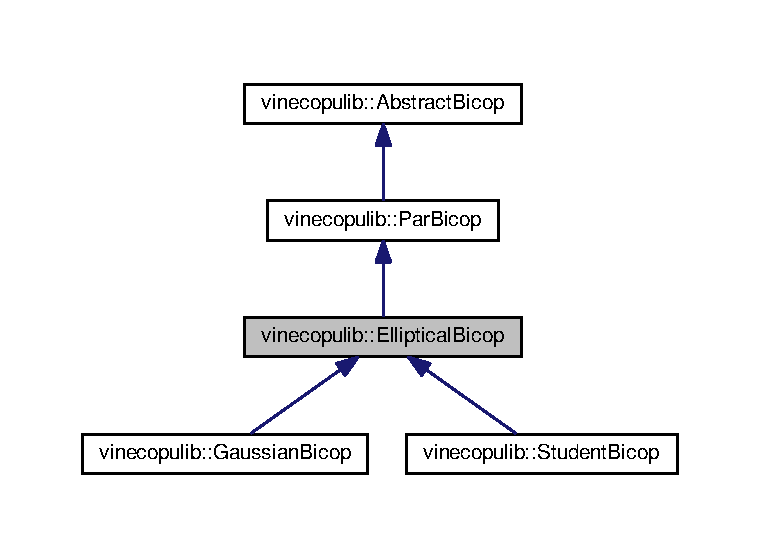
\includegraphics[width=350pt]{classvinecopulib_1_1_elliptical_bicop__inherit__graph}
\end{center}
\end{figure}


Collaboration diagram for vinecopulib\+:\+:Elliptical\+Bicop\+:\nopagebreak
\begin{figure}[H]
\begin{center}
\leavevmode
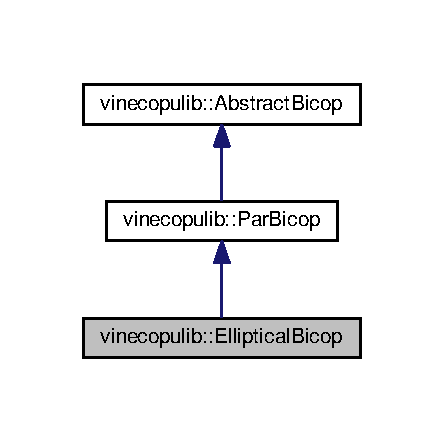
\includegraphics[width=213pt]{classvinecopulib_1_1_elliptical_bicop__coll__graph}
\end{center}
\end{figure}
\subsection*{Additional Inherited Members}


\subsection{Detailed Description}
An abstract class for elliptical copula families. 

This class is used in the implementation underlying the \hyperlink{classvinecopulib_1_1_bicop}{Bicop} class. Users should not use \hyperlink{classvinecopulib_1_1_abstract_bicop}{Abstract\+Bicop} or derived classes directly, but always work with the \hyperlink{classvinecopulib_1_1_bicop}{Bicop} interface.

Joe, Harry. Dependence modeling with copulas. C\+RC Press, 2014. 

The documentation for this class was generated from the following files\+:\begin{DoxyCompactItemize}
\item 
/home/n5/dev/cpp/vinecopulib/include/vinecopulib/bicop/elliptical.\+hpp\item 
/home/n5/dev/cpp/vinecopulib/src/bicop/elliptical.\+cpp\end{DoxyCompactItemize}

\hypertarget{classvinecopulib_1_1_frank_bicop}{}\section{vinecopulib\+:\+:Frank\+Bicop Class Reference}
\label{classvinecopulib_1_1_frank_bicop}\index{vinecopulib\+::\+Frank\+Bicop@{vinecopulib\+::\+Frank\+Bicop}}


The Frank copula.  




{\ttfamily \#include $<$frank.\+hpp$>$}



Inheritance diagram for vinecopulib\+:\+:Frank\+Bicop\+:
\nopagebreak
\begin{figure}[H]
\begin{center}
\leavevmode
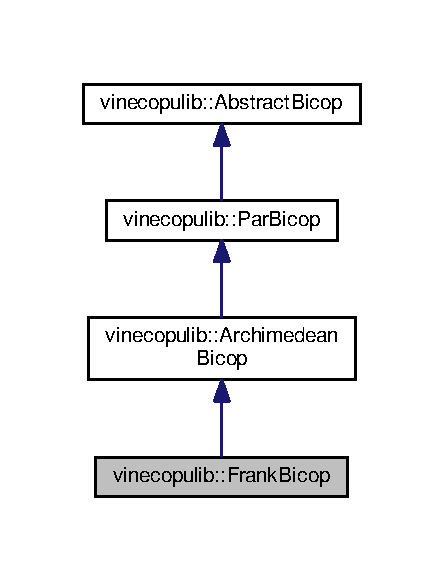
\includegraphics[width=213pt]{classvinecopulib_1_1_frank_bicop__inherit__graph}
\end{center}
\end{figure}


Collaboration diagram for vinecopulib\+:\+:Frank\+Bicop\+:
\nopagebreak
\begin{figure}[H]
\begin{center}
\leavevmode
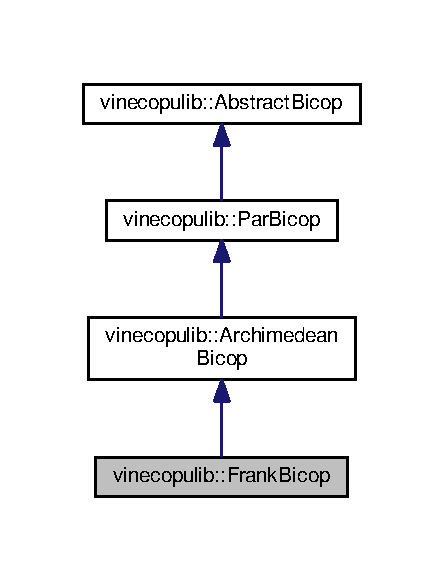
\includegraphics[width=213pt]{classvinecopulib_1_1_frank_bicop__coll__graph}
\end{center}
\end{figure}
\subsection*{Additional Inherited Members}


\subsection{Detailed Description}
The Frank copula. 

This class is used in the implementation underlying the \hyperlink{classvinecopulib_1_1_bicop}{Bicop} class. Users should not use \hyperlink{classvinecopulib_1_1_abstract_bicop}{Abstract\+Bicop} or derived classes directly, but always work with the \hyperlink{classvinecopulib_1_1_bicop}{Bicop} interface.

Joe, Harry. Dependence modeling with copulas. C\+RC Press, 2014. 

The documentation for this class was generated from the following files\+:\begin{DoxyCompactItemize}
\item 
/home/n5/dev/cpp/vinecopulib/include/bicop/frank.\+hpp\item 
/home/n5/dev/cpp/vinecopulib/src/bicop/frank.\+cpp\end{DoxyCompactItemize}

\hypertarget{classvinecopulib_1_1_gaussian_bicop}{}\section{vinecopulib\+:\+:Gaussian\+Bicop Class Reference}
\label{classvinecopulib_1_1_gaussian_bicop}\index{vinecopulib\+::\+Gaussian\+Bicop@{vinecopulib\+::\+Gaussian\+Bicop}}


The Gaussian copula.  




{\ttfamily \#include $<$gaussian.\+hpp$>$}



Inheritance diagram for vinecopulib\+:\+:Gaussian\+Bicop\+:\nopagebreak
\begin{figure}[H]
\begin{center}
\leavevmode
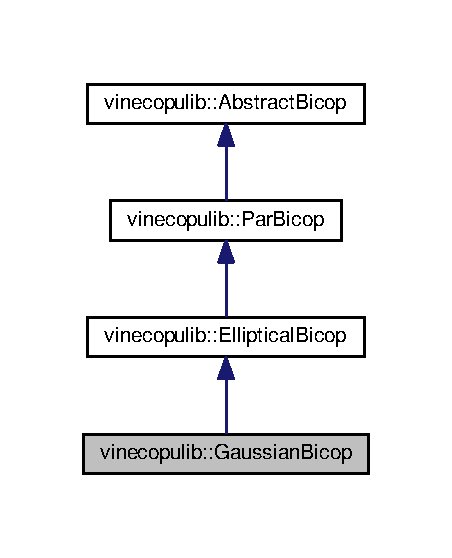
\includegraphics[width=217pt]{classvinecopulib_1_1_gaussian_bicop__inherit__graph}
\end{center}
\end{figure}


Collaboration diagram for vinecopulib\+:\+:Gaussian\+Bicop\+:\nopagebreak
\begin{figure}[H]
\begin{center}
\leavevmode
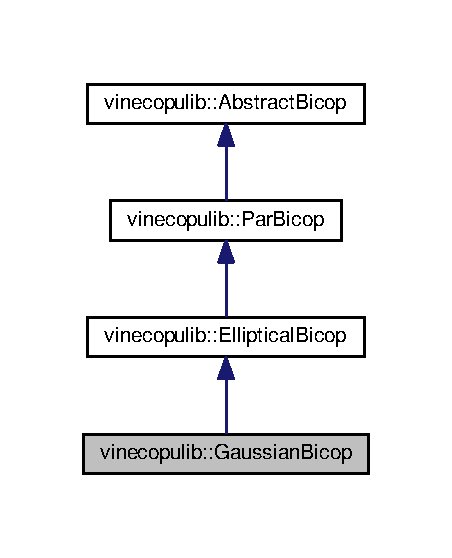
\includegraphics[width=217pt]{classvinecopulib_1_1_gaussian_bicop__coll__graph}
\end{center}
\end{figure}
\subsection*{Additional Inherited Members}


\subsection{Detailed Description}
The Gaussian copula. 

This class is used in the implementation underlying the \hyperlink{classvinecopulib_1_1_bicop}{Bicop} class. Users should not use \hyperlink{classvinecopulib_1_1_abstract_bicop}{Abstract\+Bicop} or derived classes directly, but always work with the \hyperlink{classvinecopulib_1_1_bicop}{Bicop} interface.

Joe, Harry. Dependence modeling with copulas. C\+RC Press, 2014. 

The documentation for this class was generated from the following files\+:\begin{DoxyCompactItemize}
\item 
/home/n5/dev/cpp/vinecopulib/include/vinecopulib/bicop/gaussian.\+hpp\item 
/home/n5/dev/cpp/vinecopulib/src/bicop/gaussian.\+cpp\end{DoxyCompactItemize}

\hypertarget{classvinecopulib_1_1_gumbel_bicop}{\section{vinecopulib\+:\+:Gumbel\+Bicop Class Reference}
\label{classvinecopulib_1_1_gumbel_bicop}\index{vinecopulib\+::\+Gumbel\+Bicop@{vinecopulib\+::\+Gumbel\+Bicop}}
}


The Gumbel copula.  




{\ttfamily \#include $<$gumbel.\+hpp$>$}



Inheritance diagram for vinecopulib\+:\+:Gumbel\+Bicop\+:\nopagebreak
\begin{figure}[H]
\begin{center}
\leavevmode
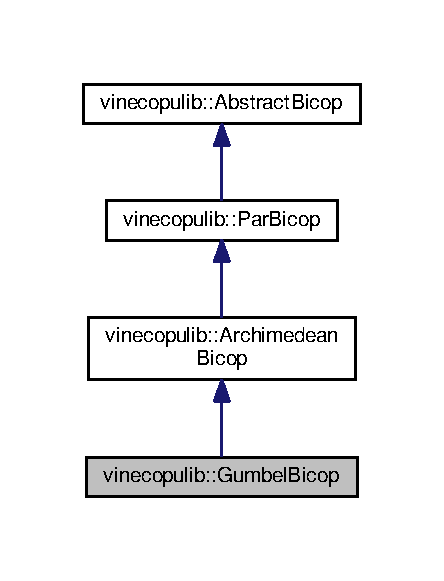
\includegraphics[width=212pt]{classvinecopulib_1_1_gumbel_bicop__inherit__graph}
\end{center}
\end{figure}


Collaboration diagram for vinecopulib\+:\+:Gumbel\+Bicop\+:\nopagebreak
\begin{figure}[H]
\begin{center}
\leavevmode
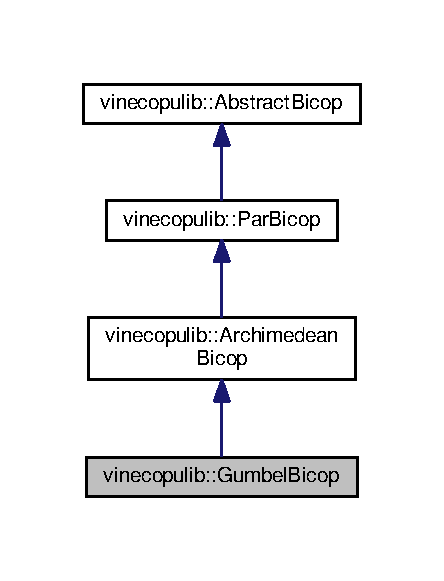
\includegraphics[width=212pt]{classvinecopulib_1_1_gumbel_bicop__coll__graph}
\end{center}
\end{figure}
\subsection*{Additional Inherited Members}


\subsection{Detailed Description}
The Gumbel copula. 

This class is used in the implementation underlying the \hyperlink{classvinecopulib_1_1_bicop}{Bicop} class. Users should not use \hyperlink{classvinecopulib_1_1_abstract_bicop}{Abstract\+Bicop} or derived classes directly, but always work with the \hyperlink{classvinecopulib_1_1_bicop}{Bicop} interface.

Joe, Harry. Dependence modeling with copulas. C\+R\+C Press, 2014. 

The documentation for this class was generated from the following files\+:\begin{DoxyCompactItemize}
\item 
vinecopulib/include/vinecopulib/bicop/gumbel.\+hpp\item 
vinecopulib/src/bicop/gumbel.\+cpp\end{DoxyCompactItemize}

\hypertarget{classvinecopulib_1_1_indep_bicop}{}\section{vinecopulib\+:\+:Indep\+Bicop Class Reference}
\label{classvinecopulib_1_1_indep_bicop}\index{vinecopulib\+::\+Indep\+Bicop@{vinecopulib\+::\+Indep\+Bicop}}


The independence copula.  




{\ttfamily \#include $<$indep.\+hpp$>$}



Inheritance diagram for vinecopulib\+:\+:Indep\+Bicop\+:\nopagebreak
\begin{figure}[H]
\begin{center}
\leavevmode
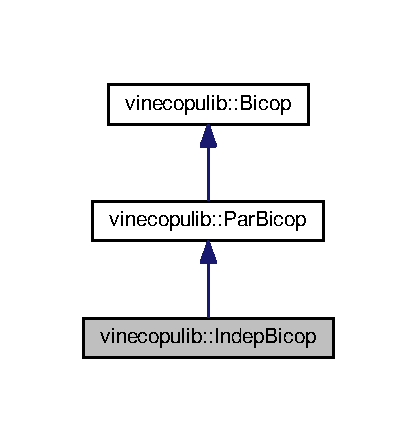
\includegraphics[width=213pt]{classvinecopulib_1_1_indep_bicop__inherit__graph}
\end{center}
\end{figure}


Collaboration diagram for vinecopulib\+:\+:Indep\+Bicop\+:\nopagebreak
\begin{figure}[H]
\begin{center}
\leavevmode
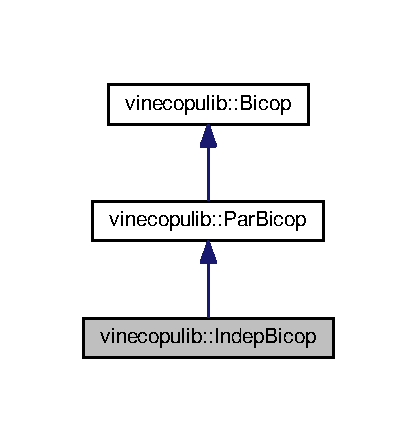
\includegraphics[width=213pt]{classvinecopulib_1_1_indep_bicop__coll__graph}
\end{center}
\end{figure}
\subsection*{Additional Inherited Members}


\subsection{Detailed Description}
The independence copula. 

This class is used in the implementation underlying the \hyperlink{classvinecopulib_1_1_bicop}{Bicop} class. Users should not use \hyperlink{classvinecopulib_1_1_abstract_bicop}{Abstract\+Bicop} or derived classes directly, but always work with the \hyperlink{classvinecopulib_1_1_bicop}{Bicop} interface.

Joe, Harry. Dependence modeling with copulas. C\+RC Press, 2014. 

The documentation for this class was generated from the following files\+:\begin{DoxyCompactItemize}
\item 
/home/n5/dev/cpp/vinecopulib/include/vinecopulib/bicop/indep.\+hpp\item 
/home/n5/dev/cpp/vinecopulib/src/bicop/indep.\+cpp\end{DoxyCompactItemize}

\hypertarget{classvinecopulib_1_1_interpolation_grid}{}\section{vinecopulib\+:\+:Interpolation\+Grid Class Reference}
\label{classvinecopulib_1_1_interpolation_grid}\index{vinecopulib\+::\+Interpolation\+Grid@{vinecopulib\+::\+Interpolation\+Grid}}


{\ttfamily \#include $<$interpolation\+\_\+grid.\+hpp$>$}

\subsection*{Public Member Functions}
\begin{DoxyCompactItemize}
\item 
\hyperlink{classvinecopulib_1_1_interpolation_grid_a9e63e4af3a252454eeae6df38fd8e0ca}{Interpolation\+Grid} (const Eigen\+::\+Vector\+Xd \&grid\+\_\+points, const Eigen\+::\+Matrix\+Xd \&values)
\item 
void {\bfseries flip} ()\hypertarget{classvinecopulib_1_1_interpolation_grid_a8dc18717a2e8dfe5b157571805a25dab}{}\label{classvinecopulib_1_1_interpolation_grid_a8dc18717a2e8dfe5b157571805a25dab}

\item 
Eigen\+::\+Vector\+Xd \hyperlink{classvinecopulib_1_1_interpolation_grid_a7fe207d7f864d2b05654c5efb5e27f35}{interpolate} (const Eigen\+::\+Matrix\+Xd \&x)
\item 
Eigen\+::\+Vector\+Xd \hyperlink{classvinecopulib_1_1_interpolation_grid_aa1811201ba71d8c3375b8e42df6f673a}{intergrate\+\_\+1d} (const Eigen\+::\+Matrix\+Xd \&u, const int \&cond\+\_\+var)
\item 
Eigen\+::\+Vector\+Xd \hyperlink{classvinecopulib_1_1_interpolation_grid_a087c7e9b9c6087b6cbbb8ba7b7292582}{inv\+\_\+intergrate\+\_\+1d} (const Eigen\+::\+Matrix\+Xd \&u, const int \&cond\+\_\+var)
\end{DoxyCompactItemize}


\subsection{Detailed Description}
A class for cubic spline interpolation of bivariate copulas

The class is used for implementing kernel estimators. It makes storing the observations obsolete and allows for fast numerical integration. 

\subsection{Constructor \& Destructor Documentation}
\index{vinecopulib\+::\+Interpolation\+Grid@{vinecopulib\+::\+Interpolation\+Grid}!Interpolation\+Grid@{Interpolation\+Grid}}
\index{Interpolation\+Grid@{Interpolation\+Grid}!vinecopulib\+::\+Interpolation\+Grid@{vinecopulib\+::\+Interpolation\+Grid}}
\subsubsection[{\texorpdfstring{Interpolation\+Grid(const Eigen\+::\+Vector\+Xd \&grid\+\_\+points, const Eigen\+::\+Matrix\+Xd \&values)}{InterpolationGrid(const Eigen::VectorXd &grid_points, const Eigen::MatrixXd &values)}}]{\setlength{\rightskip}{0pt plus 5cm}vinecopulib\+::\+Interpolation\+Grid\+::\+Interpolation\+Grid (
\begin{DoxyParamCaption}
\item[{const Eigen\+::\+Vector\+Xd \&}]{grid\+\_\+points, }
\item[{const Eigen\+::\+Matrix\+Xd \&}]{values}
\end{DoxyParamCaption}
)}\hypertarget{classvinecopulib_1_1_interpolation_grid_a9e63e4af3a252454eeae6df38fd8e0ca}{}\label{classvinecopulib_1_1_interpolation_grid_a9e63e4af3a252454eeae6df38fd8e0ca}
Constructor


\begin{DoxyParams}{Parameters}
{\em grid\+\_\+points} & an ascending sequence of grid\+\_\+points; used in both dimensions. \\
\hline
{\em values} & a dxd matrix of copula density values evaluated at (grid\+\_\+points\+\_\+i, grid\+\_\+points\+\_\+j). \\
\hline
\end{DoxyParams}


\subsection{Member Function Documentation}
\index{vinecopulib\+::\+Interpolation\+Grid@{vinecopulib\+::\+Interpolation\+Grid}!intergrate\+\_\+1d@{intergrate\+\_\+1d}}
\index{intergrate\+\_\+1d@{intergrate\+\_\+1d}!vinecopulib\+::\+Interpolation\+Grid@{vinecopulib\+::\+Interpolation\+Grid}}
\subsubsection[{\texorpdfstring{intergrate\+\_\+1d(const Eigen\+::\+Matrix\+Xd \&u, const int \&cond\+\_\+var)}{intergrate_1d(const Eigen::MatrixXd &u, const int &cond_var)}}]{\setlength{\rightskip}{0pt plus 5cm}Eigen\+::\+Vector\+Xd vinecopulib\+::\+Interpolation\+Grid\+::intergrate\+\_\+1d (
\begin{DoxyParamCaption}
\item[{const Eigen\+::\+Matrix\+Xd \&}]{u, }
\item[{const int \&}]{cond\+\_\+var}
\end{DoxyParamCaption}
)}\hypertarget{classvinecopulib_1_1_interpolation_grid_aa1811201ba71d8c3375b8e42df6f673a}{}\label{classvinecopulib_1_1_interpolation_grid_aa1811201ba71d8c3375b8e42df6f673a}
Integrate the grid along one axis


\begin{DoxyParams}{Parameters}
{\em u} & mx2 matrix of evaluation points \\
\hline
{\em cond\+\_\+var} & either 1 or 2; the axis considered fixed. \\
\hline
\end{DoxyParams}
\index{vinecopulib\+::\+Interpolation\+Grid@{vinecopulib\+::\+Interpolation\+Grid}!interpolate@{interpolate}}
\index{interpolate@{interpolate}!vinecopulib\+::\+Interpolation\+Grid@{vinecopulib\+::\+Interpolation\+Grid}}
\subsubsection[{\texorpdfstring{interpolate(const Eigen\+::\+Matrix\+Xd \&x)}{interpolate(const Eigen::MatrixXd &x)}}]{\setlength{\rightskip}{0pt plus 5cm}Eigen\+::\+Vector\+Xd vinecopulib\+::\+Interpolation\+Grid\+::interpolate (
\begin{DoxyParamCaption}
\item[{const Eigen\+::\+Matrix\+Xd \&}]{x}
\end{DoxyParamCaption}
)}\hypertarget{classvinecopulib_1_1_interpolation_grid_a7fe207d7f864d2b05654c5efb5e27f35}{}\label{classvinecopulib_1_1_interpolation_grid_a7fe207d7f864d2b05654c5efb5e27f35}
Interpolation in two dimensions


\begin{DoxyParams}{Parameters}
{\em x} & mx2 matrix of evaluation points. \\
\hline
\end{DoxyParams}
\index{vinecopulib\+::\+Interpolation\+Grid@{vinecopulib\+::\+Interpolation\+Grid}!inv\+\_\+intergrate\+\_\+1d@{inv\+\_\+intergrate\+\_\+1d}}
\index{inv\+\_\+intergrate\+\_\+1d@{inv\+\_\+intergrate\+\_\+1d}!vinecopulib\+::\+Interpolation\+Grid@{vinecopulib\+::\+Interpolation\+Grid}}
\subsubsection[{\texorpdfstring{inv\+\_\+intergrate\+\_\+1d(const Eigen\+::\+Matrix\+Xd \&u, const int \&cond\+\_\+var)}{inv_intergrate_1d(const Eigen::MatrixXd &u, const int &cond_var)}}]{\setlength{\rightskip}{0pt plus 5cm}Eigen\+::\+Vector\+Xd vinecopulib\+::\+Interpolation\+Grid\+::inv\+\_\+intergrate\+\_\+1d (
\begin{DoxyParamCaption}
\item[{const Eigen\+::\+Matrix\+Xd \&}]{u, }
\item[{const int \&}]{cond\+\_\+var}
\end{DoxyParamCaption}
)}\hypertarget{classvinecopulib_1_1_interpolation_grid_a087c7e9b9c6087b6cbbb8ba7b7292582}{}\label{classvinecopulib_1_1_interpolation_grid_a087c7e9b9c6087b6cbbb8ba7b7292582}
Inverse of integral along one axis of the grid


\begin{DoxyParams}{Parameters}
{\em u} & mx2 matrix of evaluation points \\
\hline
{\em cond\+\_\+var} & either 1 or 2; the axis considered fixed. \\
\hline
\end{DoxyParams}


The documentation for this class was generated from the following files\+:\begin{DoxyCompactItemize}
\item 
/home/n5/dev/cpp/vinecopulib/include/misc/interpolation\+\_\+grid.\+hpp\item 
/home/n5/dev/cpp/vinecopulib/src/misc/interpolation\+\_\+grid.\+cpp\end{DoxyCompactItemize}

\hypertarget{classvinecopulib_1_1_joe_bicop}{}\section{vinecopulib\+:\+:Joe\+Bicop Class Reference}
\label{classvinecopulib_1_1_joe_bicop}\index{vinecopulib\+::\+Joe\+Bicop@{vinecopulib\+::\+Joe\+Bicop}}


The Joe copula.  




{\ttfamily \#include $<$joe.\+hpp$>$}



Inheritance diagram for vinecopulib\+:\+:Joe\+Bicop\+:\nopagebreak
\begin{figure}[H]
\begin{center}
\leavevmode
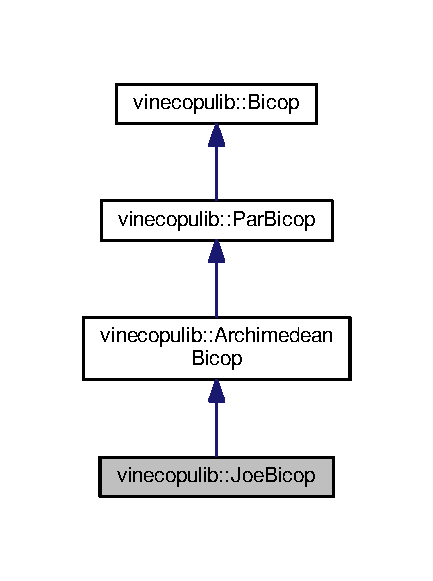
\includegraphics[width=213pt]{classvinecopulib_1_1_joe_bicop__inherit__graph}
\end{center}
\end{figure}


Collaboration diagram for vinecopulib\+:\+:Joe\+Bicop\+:\nopagebreak
\begin{figure}[H]
\begin{center}
\leavevmode
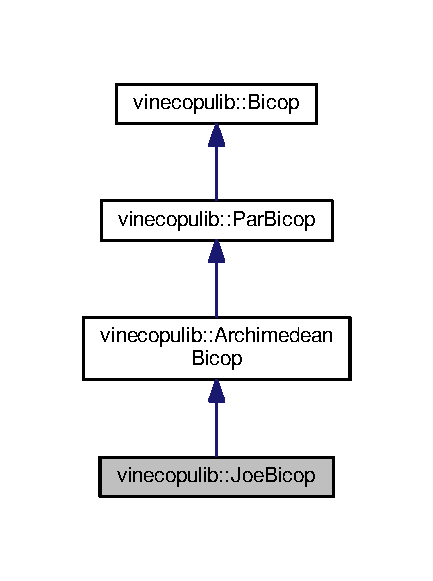
\includegraphics[width=213pt]{classvinecopulib_1_1_joe_bicop__coll__graph}
\end{center}
\end{figure}
\subsection*{Additional Inherited Members}


\subsection{Detailed Description}
The Joe copula. 

This class is used in the implementation underlying the \hyperlink{classvinecopulib_1_1_bicop}{Bicop} class. Users should not use \hyperlink{classvinecopulib_1_1_abstract_bicop}{Abstract\+Bicop} or derived classes directly, but always work with the \hyperlink{classvinecopulib_1_1_bicop}{Bicop} interface.

Joe, Harry. Dependence modeling with copulas. C\+RC Press, 2014. 

The documentation for this class was generated from the following files\+:\begin{DoxyCompactItemize}
\item 
/home/n5/dev/cpp/vinecopulib/include/vinecopulib/bicop/joe.\+hpp\item 
/home/n5/dev/cpp/vinecopulib/src/bicop/joe.\+cpp\end{DoxyCompactItemize}

\hypertarget{classvinecopulib_1_1_kernel_bicop}{}\section{vinecopulib\+:\+:Kernel\+Bicop Class Reference}
\label{classvinecopulib_1_1_kernel_bicop}\index{vinecopulib\+::\+Kernel\+Bicop@{vinecopulib\+::\+Kernel\+Bicop}}


An abstract class for kernel copulas.  




{\ttfamily \#include $<$kernel.\+hpp$>$}



Inheritance diagram for vinecopulib\+:\+:Kernel\+Bicop\+:
\nopagebreak
\begin{figure}[H]
\begin{center}
\leavevmode
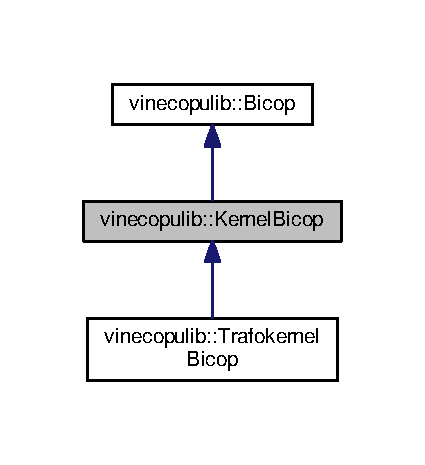
\includegraphics[width=213pt]{classvinecopulib_1_1_kernel_bicop__inherit__graph}
\end{center}
\end{figure}


Collaboration diagram for vinecopulib\+:\+:Kernel\+Bicop\+:
\nopagebreak
\begin{figure}[H]
\begin{center}
\leavevmode
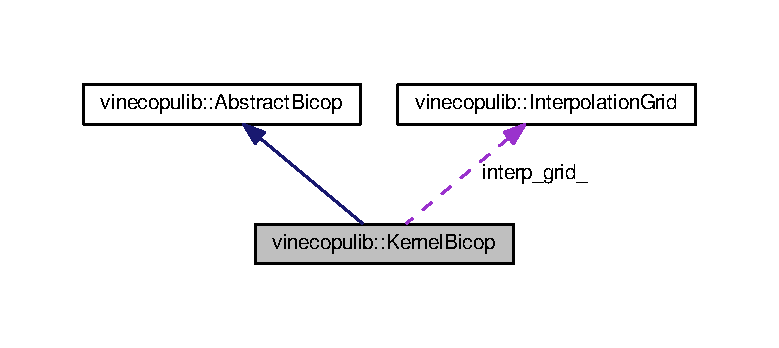
\includegraphics[width=350pt]{classvinecopulib_1_1_kernel_bicop__coll__graph}
\end{center}
\end{figure}
\subsection*{Protected Member Functions}
\begin{DoxyCompactItemize}
\item 
Eigen\+::\+Vector\+Xd {\bfseries pdf} (const Eigen\+::\+Matrix$<$ double, Eigen\+::\+Dynamic, 2 $>$ \&u)\hypertarget{classvinecopulib_1_1_kernel_bicop_a307624ad91ab1fd38ae7933fab0a5f6a}{}\label{classvinecopulib_1_1_kernel_bicop_a307624ad91ab1fd38ae7933fab0a5f6a}

\item 
Eigen\+::\+Vector\+Xd {\bfseries hfunc1} (const Eigen\+::\+Matrix$<$ double, Eigen\+::\+Dynamic, 2 $>$ \&u)\hypertarget{classvinecopulib_1_1_kernel_bicop_a08a6961d233bc977e583b5253c6089dc}{}\label{classvinecopulib_1_1_kernel_bicop_a08a6961d233bc977e583b5253c6089dc}

\item 
Eigen\+::\+Vector\+Xd {\bfseries hfunc2} (const Eigen\+::\+Matrix$<$ double, Eigen\+::\+Dynamic, 2 $>$ \&u)\hypertarget{classvinecopulib_1_1_kernel_bicop_ae4983795f404cca9c4a6af15d41b104a}{}\label{classvinecopulib_1_1_kernel_bicop_ae4983795f404cca9c4a6af15d41b104a}

\item 
Eigen\+::\+Vector\+Xd {\bfseries hinv1} (const Eigen\+::\+Matrix$<$ double, Eigen\+::\+Dynamic, 2 $>$ \&u)\hypertarget{classvinecopulib_1_1_kernel_bicop_aca726ccdf9a1551fb342dd7e60de1f84}{}\label{classvinecopulib_1_1_kernel_bicop_aca726ccdf9a1551fb342dd7e60de1f84}

\item 
Eigen\+::\+Vector\+Xd {\bfseries hinv2} (const Eigen\+::\+Matrix$<$ double, Eigen\+::\+Dynamic, 2 $>$ \&u)\hypertarget{classvinecopulib_1_1_kernel_bicop_a809dc2c7f0a67d217e0fe9651a625a6b}{}\label{classvinecopulib_1_1_kernel_bicop_a809dc2c7f0a67d217e0fe9651a625a6b}

\item 
double {\bfseries parameters\+\_\+to\+\_\+tau} (const Eigen\+::\+Vector\+Xd \&)\hypertarget{classvinecopulib_1_1_kernel_bicop_a1c00a74e12159b2c06487cf1b3ccff00}{}\label{classvinecopulib_1_1_kernel_bicop_a1c00a74e12159b2c06487cf1b3ccff00}

\item 
Eigen\+::\+Matrix\+Xd {\bfseries tau\+\_\+to\+\_\+parameters} (const double \&tau)\hypertarget{classvinecopulib_1_1_kernel_bicop_a510489f8f985c04c4f692e12ab2d1bf0}{}\label{classvinecopulib_1_1_kernel_bicop_a510489f8f985c04c4f692e12ab2d1bf0}

\item 
double {\bfseries calculate\+\_\+npars} ()\hypertarget{classvinecopulib_1_1_kernel_bicop_a33f736d5f443399f1f4dbe54b386aba3}{}\label{classvinecopulib_1_1_kernel_bicop_a33f736d5f443399f1f4dbe54b386aba3}

\item 
void {\bfseries flip} ()\hypertarget{classvinecopulib_1_1_kernel_bicop_abc23a81271f970b9c99dd6ed727c170f}{}\label{classvinecopulib_1_1_kernel_bicop_abc23a81271f970b9c99dd6ed727c170f}

\end{DoxyCompactItemize}
\subsection*{Protected Attributes}
\begin{DoxyCompactItemize}
\item 
\hyperlink{classvinecopulib_1_1_interpolation_grid}{Interpolation\+Grid} {\bfseries interp\+\_\+grid\+\_\+}\hypertarget{classvinecopulib_1_1_kernel_bicop_aa8cfe1dd0786d692562252de05c46588}{}\label{classvinecopulib_1_1_kernel_bicop_aa8cfe1dd0786d692562252de05c46588}

\item 
double {\bfseries npars\+\_\+}\hypertarget{classvinecopulib_1_1_kernel_bicop_a1b49a0a2630e71079c08ebdca79b06b6}{}\label{classvinecopulib_1_1_kernel_bicop_a1b49a0a2630e71079c08ebdca79b06b6}

\end{DoxyCompactItemize}
\subsection*{Additional Inherited Members}


\subsection{Detailed Description}
An abstract class for kernel copulas. 

Evaluation functions of kernel estimators are implemented efficiently using spline interpolation, see Nagler (2016).

This class is used in the implementation underlying the \hyperlink{classvinecopulib_1_1_bicop}{Bicop} class. Users should not use \hyperlink{classvinecopulib_1_1_abstract_bicop}{Abstract\+Bicop} or derived classes directly, but always work with the \hyperlink{classvinecopulib_1_1_bicop}{Bicop} interface.

Nagler, Thomas. {\itshape kdecopula\+: An R Package for the Kernel Estimation of Copula Densities}. ar\+Xiv\+:1603.\+04229 \mbox{[}stat.\+CO\mbox{]}, 2016 

The documentation for this class was generated from the following files\+:\begin{DoxyCompactItemize}
\item 
/home/n5/dev/cpp/vinecopulib/include/bicop/kernel.\+hpp\item 
/home/n5/dev/cpp/vinecopulib/src/bicop/kernel.\+cpp\end{DoxyCompactItemize}

\hypertarget{classvinecopulib_1_1_par_bicop}{}\section{vinecopulib\+:\+:Par\+Bicop Class Reference}
\label{classvinecopulib_1_1_par_bicop}\index{vinecopulib\+::\+Par\+Bicop@{vinecopulib\+::\+Par\+Bicop}}


Inheritance diagram for vinecopulib\+:\+:Par\+Bicop\+:\nopagebreak
\begin{figure}[H]
\begin{center}
\leavevmode
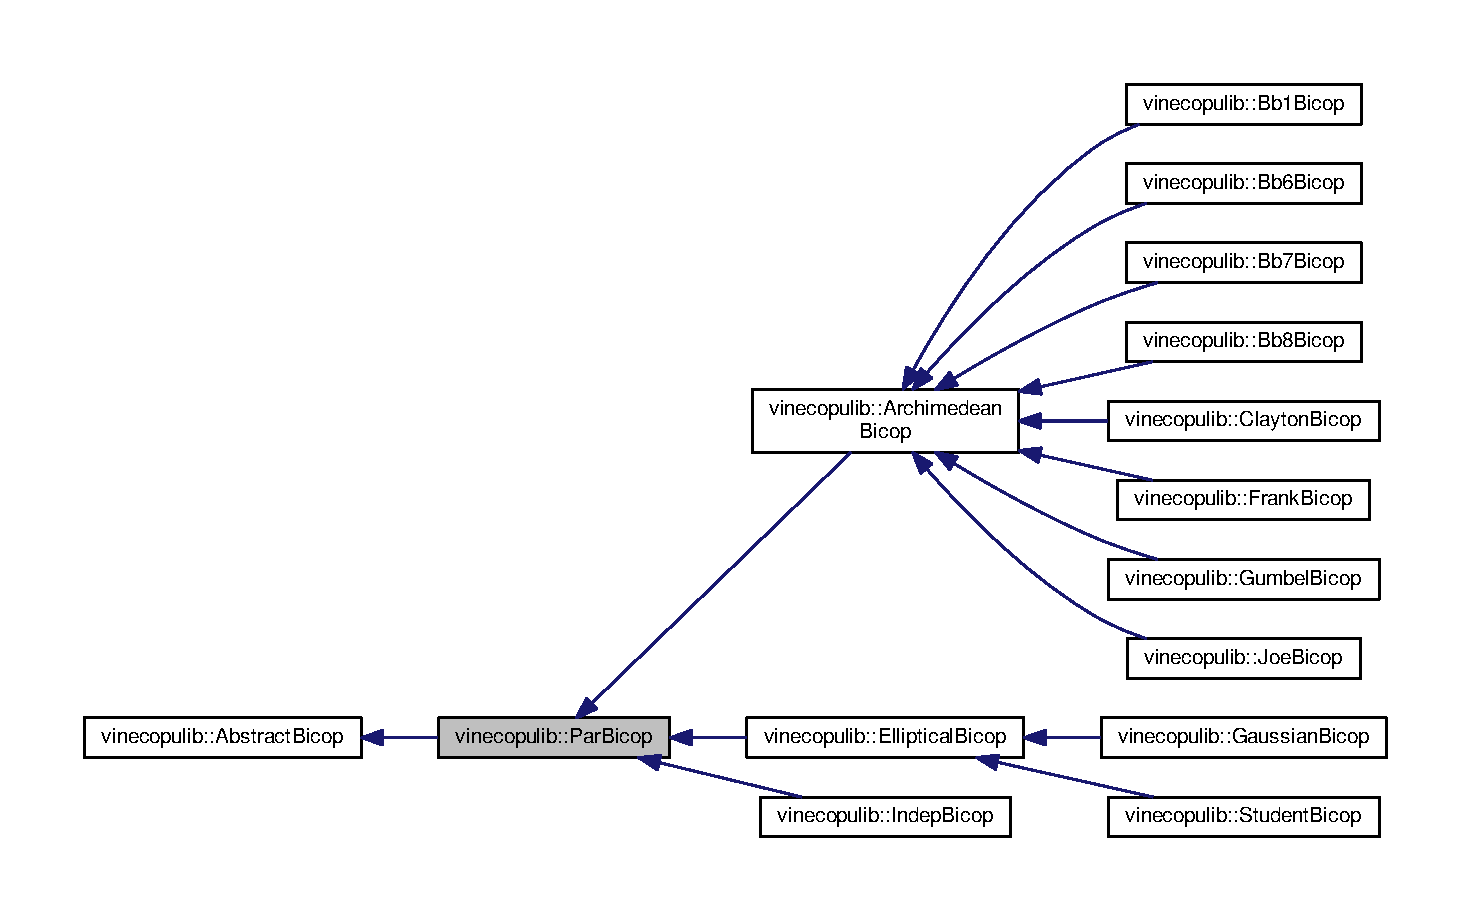
\includegraphics[width=350pt]{classvinecopulib_1_1_par_bicop__inherit__graph}
\end{center}
\end{figure}


Collaboration diagram for vinecopulib\+:\+:Par\+Bicop\+:\nopagebreak
\begin{figure}[H]
\begin{center}
\leavevmode
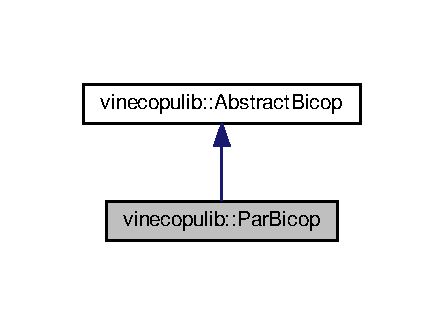
\includegraphics[width=191pt]{classvinecopulib_1_1_par_bicop__coll__graph}
\end{center}
\end{figure}
\subsection*{Additional Inherited Members}


The documentation for this class was generated from the following files\+:\begin{DoxyCompactItemize}
\item 
/home/n5/dev/cpp/vinecopulib/include/bicop\+\_\+parametric.\+hpp\item 
/home/n5/dev/cpp/vinecopulib/src/bicop\+\_\+parametric.\+cpp\end{DoxyCompactItemize}

\hypertarget{classvinecopulib_1_1_r_vine_matrix}{\section{vinecopulib\+:\+:R\+Vine\+Matrix Class Reference}
\label{classvinecopulib_1_1_r_vine_matrix}\index{vinecopulib\+::\+R\+Vine\+Matrix@{vinecopulib\+::\+R\+Vine\+Matrix}}
}


A class for regular vine matrices.  




{\ttfamily \#include $<$rvine\+\_\+matrix.\+hpp$>$}

\subsection*{Public Member Functions}
\begin{DoxyCompactItemize}
\item 
\hyperlink{classvinecopulib_1_1_r_vine_matrix_a966316e211937ae11e840ef7540a492f}{R\+Vine\+Matrix} (const Eigen\+::\+Matrix$<$ size\+\_\+t, Eigen\+::\+Dynamic, Eigen\+::\+Dynamic $>$ \&matrix, bool check=true)
\item 
\hypertarget{classvinecopulib_1_1_r_vine_matrix_a37c79233fca1e56e1535cbb37f8d3177}{Eigen\+::\+Matrix$<$ size\+\_\+t, \\*
Eigen\+::\+Dynamic, Eigen\+::\+Dynamic $>$ \hyperlink{classvinecopulib_1_1_r_vine_matrix_a37c79233fca1e56e1535cbb37f8d3177}{get\+\_\+matrix} () const }\label{classvinecopulib_1_1_r_vine_matrix_a37c79233fca1e56e1535cbb37f8d3177}

\begin{DoxyCompactList}\small\item\em extract the matrix. \end{DoxyCompactList}\item 
\hypertarget{classvinecopulib_1_1_r_vine_matrix_a71554c734c3cbb4c066c1f17fe94a284}{Eigen\+::\+Matrix$<$ size\+\_\+t, \\*
Eigen\+::\+Dynamic, 1 $>$ \hyperlink{classvinecopulib_1_1_r_vine_matrix_a71554c734c3cbb4c066c1f17fe94a284}{get\+\_\+order} () const }\label{classvinecopulib_1_1_r_vine_matrix_a71554c734c3cbb4c066c1f17fe94a284}

\begin{DoxyCompactList}\small\item\em extracts the variable order in the R-\/vine. \end{DoxyCompactList}\item 
Eigen\+::\+Matrix$<$ size\+\_\+t, \\*
Eigen\+::\+Dynamic, Eigen\+::\+Dynamic $>$ \hyperlink{classvinecopulib_1_1_r_vine_matrix_a4e63d8b01e1d89284ca28192676b8a3f}{in\+\_\+natural\+\_\+order} () const 
\item 
Eigen\+::\+Matrix$<$ size\+\_\+t, \\*
Eigen\+::\+Dynamic, Eigen\+::\+Dynamic $>$ \hyperlink{classvinecopulib_1_1_r_vine_matrix_aef8bbe14451d023e1c9c113e3812f574}{get\+\_\+max\+\_\+matrix} () const 
\item 
\hyperlink{namespacevinecopulib_1_1tools__eigen_a2fcd63009df35741859f44f1e41931f9}{Matrix\+Xb} \hyperlink{classvinecopulib_1_1_r_vine_matrix_a6303fc1f643fdf793c867ca7e08e42bc}{get\+\_\+needed\+\_\+hfunc1} () const 
\item 
\hyperlink{namespacevinecopulib_1_1tools__eigen_a2fcd63009df35741859f44f1e41931f9}{Matrix\+Xb} \hyperlink{classvinecopulib_1_1_r_vine_matrix_a7ac32cf10a966ba567142e9b36106746}{get\+\_\+needed\+\_\+hfunc2} () const 
\end{DoxyCompactItemize}
\subsection*{Static Public Member Functions}
\begin{DoxyCompactItemize}
\item 
static Eigen\+::\+Matrix$<$ size\+\_\+t, \\*
Eigen\+::\+Dynamic, Eigen\+::\+Dynamic $>$ \hyperlink{classvinecopulib_1_1_r_vine_matrix_ad523b84e2ea41eba4eb982eb9b39471b}{construct\+\_\+d\+\_\+vine\+\_\+matrix} (const Eigen\+::\+Matrix$<$ size\+\_\+t, Eigen\+::\+Dynamic, 1 $>$ \&order)
\end{DoxyCompactItemize}


\subsection{Detailed Description}
A class for regular vine matrices. 

A regular vine (R-\/vine) matrix encodes the structure of a vine. An examplary matrix is ``` 1 1 1 1 2 2 2 0 3 3 0 0 4 0 0 0 ``` which encodes the following pair-\/copulas\+: ``` \begin{TabularC}{3}
\hline
\rowcolor{lightgray}{\bf tree }&{\bf edge }&{\bf pair-\/copulas  }\\\cline{1-3}
0 &0 &{\ttfamily (4, 1)} \\\cline{1-3}
&1 &{\ttfamily (3, 1)} \\\cline{1-3}
&2 &{\ttfamily (2, 1)} \\\cline{1-3}
1 &0 &{\ttfamily (4, 2; 1)} \\\cline{1-3}
&1 &{\ttfamily (3, 2; 1)} \\\cline{1-3}
2 &0 &{\ttfamily (4, 3; 2, 1)} \\\cline{1-3}
\end{TabularC}
``{\ttfamily  Denoting by}M\mbox{[}i\mbox{]}\mbox{[}j\mbox{]}{\ttfamily the matrix entry in row}i{\ttfamily and column}j{\ttfamily  (starting at 0), the pair-\/copula index for edge}e{\ttfamily in tree}t{\ttfamily of a }d{\ttfamily dimensional vine is }(M\mbox{[}d -\/ 1 -\/ t\mbox{]}\mbox{[}e\mbox{]}, M\mbox{[}t\mbox{]}\mbox{[}e\mbox{]}; M\mbox{[}t -\/ 1\mbox{]}\mbox{[}e\mbox{]}, ..., M\mbox{[}0\mbox{]}\mbox{[}e\mbox{]})`. Less formally,
\begin{DoxyEnumerate}
\item Start with the counter-\/diagonal element of column {\ttfamily e} (first conditioned variable).
\item Jump up to the element in row {\ttfamily t} (second conditioned variable).
\item Gather all entries further up in column {\ttfamily e} (conditioning set).
\end{DoxyEnumerate}

A valid R-\/vine matrix must satisfy several conditions which are checked when {\ttfamily R\+Vine\+Matrix()} is called\+:
\begin{DoxyEnumerate}
\item The lower right triangle must only contain zeros.
\item The upper left triangle can only contain numbers between 1 and d.
\item The antidiagonal must contain the numbers 1, ..., d.
\item The antidiagonal entry of a column must not be contained in any column further to the right.
\item The entries of a column must be contained in all columns to the left.
\item The proximity condition must hold\+: For all t = 1, ..., d -\/ 2 and e = 0, ..., d -\/ t -\/ 1 there must exist an index j $>$ d, such that {\ttfamily (M\mbox{[}t, e\mbox{]}, \{M\mbox{[}0, e\mbox{]}, ..., M\mbox{[}t-\/1, e\mbox{]}\})} equals either {\ttfamily (M\mbox{[}d-\/j-\/1, j\mbox{]}, \{M\mbox{[}0, j\mbox{]}, ..., M\mbox{[}t-\/1, j\mbox{]}\})} or {\ttfamily (M\mbox{[}t-\/1, j\mbox{]}, \{M\mbox{[}d-\/j-\/1, j\mbox{]}, M\mbox{[}0, j\mbox{]}, ..., M\mbox{[}t-\/2, j\mbox{]}\})}.
\end{DoxyEnumerate}

Condition 6 already implies conditions 2-\/5, but is more difficult to check by hand. 

\subsection{Constructor \& Destructor Documentation}
\hypertarget{classvinecopulib_1_1_r_vine_matrix_a966316e211937ae11e840ef7540a492f}{\index{vinecopulib\+::\+R\+Vine\+Matrix@{vinecopulib\+::\+R\+Vine\+Matrix}!R\+Vine\+Matrix@{R\+Vine\+Matrix}}
\index{R\+Vine\+Matrix@{R\+Vine\+Matrix}!vinecopulib\+::\+R\+Vine\+Matrix@{vinecopulib\+::\+R\+Vine\+Matrix}}
\subsubsection[{R\+Vine\+Matrix}]{\setlength{\rightskip}{0pt plus 5cm}vinecopulib\+::\+R\+Vine\+Matrix\+::\+R\+Vine\+Matrix (
\begin{DoxyParamCaption}
\item[{const Eigen\+::\+Matrix$<$ size\+\_\+t, Eigen\+::\+Dynamic, Eigen\+::\+Dynamic $>$ \&}]{matrix, }
\item[{bool}]{check = {\ttfamily true}}
\end{DoxyParamCaption}
)}}\label{classvinecopulib_1_1_r_vine_matrix_a966316e211937ae11e840ef7540a492f}
instantiates an \hyperlink{classvinecopulib_1_1_r_vine_matrix}{R\+Vine\+Matrix} object. 
\begin{DoxyParams}{Parameters}
{\em matrix} & a valid R-\/vine matrix. \\
\hline
{\em check} & whether the matrix shall be checked for validity. \\
\hline
\end{DoxyParams}


\subsection{Member Function Documentation}
\hypertarget{classvinecopulib_1_1_r_vine_matrix_ad523b84e2ea41eba4eb982eb9b39471b}{\index{vinecopulib\+::\+R\+Vine\+Matrix@{vinecopulib\+::\+R\+Vine\+Matrix}!construct\+\_\+d\+\_\+vine\+\_\+matrix@{construct\+\_\+d\+\_\+vine\+\_\+matrix}}
\index{construct\+\_\+d\+\_\+vine\+\_\+matrix@{construct\+\_\+d\+\_\+vine\+\_\+matrix}!vinecopulib\+::\+R\+Vine\+Matrix@{vinecopulib\+::\+R\+Vine\+Matrix}}
\subsubsection[{construct\+\_\+d\+\_\+vine\+\_\+matrix}]{\setlength{\rightskip}{0pt plus 5cm}Eigen\+::\+Matrix$<$ size\+\_\+t, Eigen\+::\+Dynamic, Eigen\+::\+Dynamic $>$ vinecopulib\+::\+R\+Vine\+Matrix\+::construct\+\_\+d\+\_\+vine\+\_\+matrix (
\begin{DoxyParamCaption}
\item[{const Eigen\+::\+Matrix$<$ size\+\_\+t, Eigen\+::\+Dynamic, 1 $>$ \&}]{order}
\end{DoxyParamCaption}
)\hspace{0.3cm}{\ttfamily [static]}}}\label{classvinecopulib_1_1_r_vine_matrix_ad523b84e2ea41eba4eb982eb9b39471b}
constructs a D-\/vine matrix.

A D-\/vine is a vine where each tree is a path.


\begin{DoxyParams}{Parameters}
{\em order} & order of the variables. \\
\hline
\end{DoxyParams}
\hypertarget{classvinecopulib_1_1_r_vine_matrix_aef8bbe14451d023e1c9c113e3812f574}{\index{vinecopulib\+::\+R\+Vine\+Matrix@{vinecopulib\+::\+R\+Vine\+Matrix}!get\+\_\+max\+\_\+matrix@{get\+\_\+max\+\_\+matrix}}
\index{get\+\_\+max\+\_\+matrix@{get\+\_\+max\+\_\+matrix}!vinecopulib\+::\+R\+Vine\+Matrix@{vinecopulib\+::\+R\+Vine\+Matrix}}
\subsubsection[{get\+\_\+max\+\_\+matrix}]{\setlength{\rightskip}{0pt plus 5cm}Eigen\+::\+Matrix$<$ size\+\_\+t, Eigen\+::\+Dynamic, Eigen\+::\+Dynamic $>$ vinecopulib\+::\+R\+Vine\+Matrix\+::get\+\_\+max\+\_\+matrix (
\begin{DoxyParamCaption}
{}
\end{DoxyParamCaption}
) const}}\label{classvinecopulib_1_1_r_vine_matrix_aef8bbe14451d023e1c9c113e3812f574}
extracts the maximum matrix.

The maximum matrix is derived from an R-\/vine matrix by iteratively computing the (elementwise) maximum of a row and the row below (starting from the bottom). It is used in estimation and evaluation algorithms to find the right pseudo observations for an edge. \hypertarget{classvinecopulib_1_1_r_vine_matrix_a6303fc1f643fdf793c867ca7e08e42bc}{\index{vinecopulib\+::\+R\+Vine\+Matrix@{vinecopulib\+::\+R\+Vine\+Matrix}!get\+\_\+needed\+\_\+hfunc1@{get\+\_\+needed\+\_\+hfunc1}}
\index{get\+\_\+needed\+\_\+hfunc1@{get\+\_\+needed\+\_\+hfunc1}!vinecopulib\+::\+R\+Vine\+Matrix@{vinecopulib\+::\+R\+Vine\+Matrix}}
\subsubsection[{get\+\_\+needed\+\_\+hfunc1}]{\setlength{\rightskip}{0pt plus 5cm}{\bf Matrix\+Xb} vinecopulib\+::\+R\+Vine\+Matrix\+::get\+\_\+needed\+\_\+hfunc1 (
\begin{DoxyParamCaption}
{}
\end{DoxyParamCaption}
) const}}\label{classvinecopulib_1_1_r_vine_matrix_a6303fc1f643fdf793c867ca7e08e42bc}
extracts a matrix indicating which of the first h-\/functions are needed (it is usually not necessary to apply both h-\/functions for each pair-\/copula). \hypertarget{classvinecopulib_1_1_r_vine_matrix_a7ac32cf10a966ba567142e9b36106746}{\index{vinecopulib\+::\+R\+Vine\+Matrix@{vinecopulib\+::\+R\+Vine\+Matrix}!get\+\_\+needed\+\_\+hfunc2@{get\+\_\+needed\+\_\+hfunc2}}
\index{get\+\_\+needed\+\_\+hfunc2@{get\+\_\+needed\+\_\+hfunc2}!vinecopulib\+::\+R\+Vine\+Matrix@{vinecopulib\+::\+R\+Vine\+Matrix}}
\subsubsection[{get\+\_\+needed\+\_\+hfunc2}]{\setlength{\rightskip}{0pt plus 5cm}{\bf Matrix\+Xb} vinecopulib\+::\+R\+Vine\+Matrix\+::get\+\_\+needed\+\_\+hfunc2 (
\begin{DoxyParamCaption}
{}
\end{DoxyParamCaption}
) const}}\label{classvinecopulib_1_1_r_vine_matrix_a7ac32cf10a966ba567142e9b36106746}
extracts a matrix indicating which of the second h-\/functions are needed (it is usually not necessary to apply both h-\/functions for each pair-\/copula). \hypertarget{classvinecopulib_1_1_r_vine_matrix_a4e63d8b01e1d89284ca28192676b8a3f}{\index{vinecopulib\+::\+R\+Vine\+Matrix@{vinecopulib\+::\+R\+Vine\+Matrix}!in\+\_\+natural\+\_\+order@{in\+\_\+natural\+\_\+order}}
\index{in\+\_\+natural\+\_\+order@{in\+\_\+natural\+\_\+order}!vinecopulib\+::\+R\+Vine\+Matrix@{vinecopulib\+::\+R\+Vine\+Matrix}}
\subsubsection[{in\+\_\+natural\+\_\+order}]{\setlength{\rightskip}{0pt plus 5cm}Eigen\+::\+Matrix$<$ size\+\_\+t, Eigen\+::\+Dynamic, Eigen\+::\+Dynamic $>$ vinecopulib\+::\+R\+Vine\+Matrix\+::in\+\_\+natural\+\_\+order (
\begin{DoxyParamCaption}
{}
\end{DoxyParamCaption}
) const}}\label{classvinecopulib_1_1_r_vine_matrix_a4e63d8b01e1d89284ca28192676b8a3f}
extracts the R-\/vine matrix in natural order.

Natural order means that the counter-\/diagonal has entries (d, ..., 1). We convert to natural order by relabeling the variables. Most algorithms for estimation and evaluation assume that the R-\/vine matrix is in natural order. 

The documentation for this class was generated from the following files\+:\begin{DoxyCompactItemize}
\item 
vinecopulib/include/vinecopulib/vinecop/rvine\+\_\+matrix.\+hpp\item 
vinecopulib/src/vinecop/rvine\+\_\+matrix.\+cpp\end{DoxyCompactItemize}

\hypertarget{classvinecopulib_1_1_student_bicop}{\section{vinecopulib\+:\+:Student\+Bicop Class Reference}
\label{classvinecopulib_1_1_student_bicop}\index{vinecopulib\+::\+Student\+Bicop@{vinecopulib\+::\+Student\+Bicop}}
}


The Student t copula.  




{\ttfamily \#include $<$student.\+hpp$>$}



Inheritance diagram for vinecopulib\+:\+:Student\+Bicop\+:\nopagebreak
\begin{figure}[H]
\begin{center}
\leavevmode
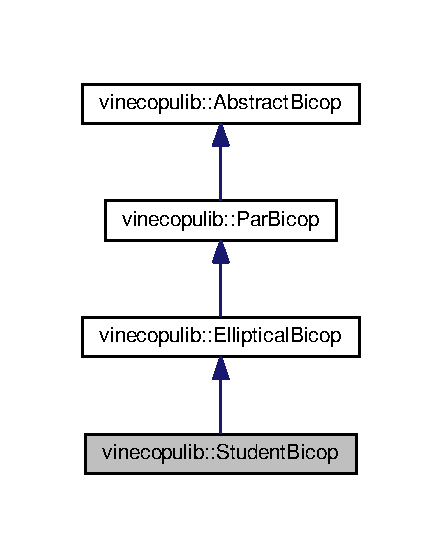
\includegraphics[width=212pt]{classvinecopulib_1_1_student_bicop__inherit__graph}
\end{center}
\end{figure}


Collaboration diagram for vinecopulib\+:\+:Student\+Bicop\+:\nopagebreak
\begin{figure}[H]
\begin{center}
\leavevmode
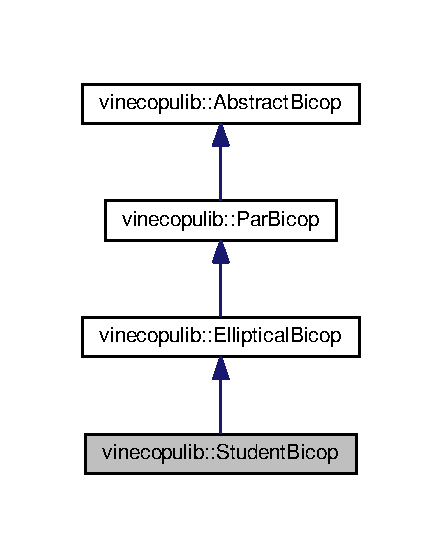
\includegraphics[width=212pt]{classvinecopulib_1_1_student_bicop__coll__graph}
\end{center}
\end{figure}
\subsection*{Additional Inherited Members}


\subsection{Detailed Description}
The Student t copula. 

This class is used in the implementation underlying the \hyperlink{classvinecopulib_1_1_bicop}{Bicop} class. Users should not use \hyperlink{classvinecopulib_1_1_abstract_bicop}{Abstract\+Bicop} or derived classes directly, but always work with the \hyperlink{classvinecopulib_1_1_bicop}{Bicop} interface.

Joe, Harry. Dependence modeling with copulas. C\+R\+C Press, 2014. 

The documentation for this class was generated from the following files\+:\begin{DoxyCompactItemize}
\item 
vinecopulib/include/vinecopulib/bicop/student.\+hpp\item 
vinecopulib/src/bicop/student.\+cpp\end{DoxyCompactItemize}

\hypertarget{classvinecopulib_1_1_trafokernel_bicop}{}\section{vinecopulib\+:\+:Trafokernel\+Bicop Class Reference}
\label{classvinecopulib_1_1_trafokernel_bicop}\index{vinecopulib\+::\+Trafokernel\+Bicop@{vinecopulib\+::\+Trafokernel\+Bicop}}


The transformation local-\/constant likelihood estimator.  




{\ttfamily \#include $<$trafokernel.\+hpp$>$}



Inheritance diagram for vinecopulib\+:\+:Trafokernel\+Bicop\+:\nopagebreak
\begin{figure}[H]
\begin{center}
\leavevmode
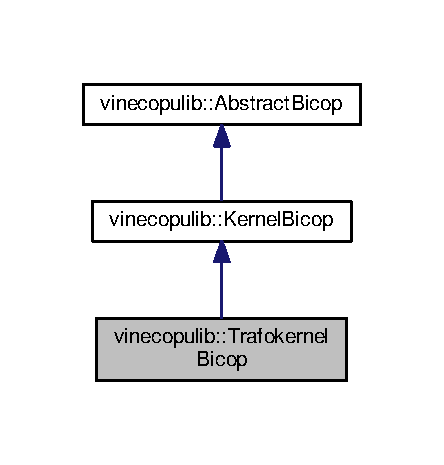
\includegraphics[width=213pt]{classvinecopulib_1_1_trafokernel_bicop__inherit__graph}
\end{center}
\end{figure}


Collaboration diagram for vinecopulib\+:\+:Trafokernel\+Bicop\+:\nopagebreak
\begin{figure}[H]
\begin{center}
\leavevmode
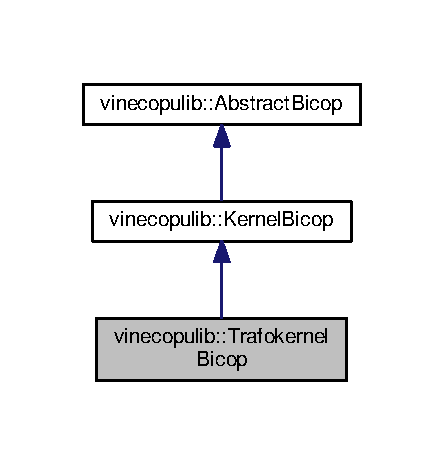
\includegraphics[width=213pt]{classvinecopulib_1_1_trafokernel_bicop__coll__graph}
\end{center}
\end{figure}
\subsection*{Additional Inherited Members}


\subsection{Detailed Description}
The transformation local-\/constant likelihood estimator. 

This class is used in the implementation underlying the \hyperlink{classvinecopulib_1_1_bicop}{Bicop} class. Users should not use \hyperlink{classvinecopulib_1_1_abstract_bicop}{Abstract\+Bicop} or derived classes directly, but always work with the \hyperlink{classvinecopulib_1_1_bicop}{Bicop} interface.

Nagler, Thomas. {\itshape kdecopula\+: An R Package for the Kernel Estimation of Copula Densities}. ar\+Xiv\+:1603.\+04229 \mbox{[}stat.\+CO\mbox{]}, 2016 

The documentation for this class was generated from the following files\+:\begin{DoxyCompactItemize}
\item 
/home/n5/dev/cpp/vinecopulib/include/bicop/trafokernel.\+hpp\item 
/home/n5/dev/cpp/vinecopulib/src/bicop/trafokernel.\+cpp\end{DoxyCompactItemize}

\hypertarget{classvinecopulib_1_1_vinecop}{}\section{vinecopulib\+:\+:Vinecop Class Reference}
\label{classvinecopulib_1_1_vinecop}\index{vinecopulib\+::\+Vinecop@{vinecopulib\+::\+Vinecop}}


A class for vine copula models.  




{\ttfamily \#include $<$class.\+hpp$>$}

\subsection*{Public Member Functions}
\begin{DoxyCompactItemize}
\item 
\hyperlink{classvinecopulib_1_1_vinecop_a391541e2795d06a848d5a17fe3496a63}{Vinecop} (size\+\_\+t d)
\item 
\hyperlink{classvinecopulib_1_1_vinecop_ab44ab72bb062123dabe8c1a5c569f0c0}{Vinecop} (const Eigen\+::\+Matrix$<$ size\+\_\+t, Eigen\+::\+Dynamic, Eigen\+::\+Dynamic $>$ \&matrix)
\item 
\hyperlink{classvinecopulib_1_1_vinecop_a4e6f60c2ddb191f0fe083dda346d0dd1}{Vinecop} (const std\+::vector$<$ std\+::vector$<$ \hyperlink{classvinecopulib_1_1_bicop}{Bicop} $>$$>$ \&pair\+\_\+copulas, const Eigen\+::\+Matrix$<$ size\+\_\+t, Eigen\+::\+Dynamic, Eigen\+::\+Dynamic $>$ \&matrix)
\item 
\hyperlink{classvinecopulib_1_1_vinecop_a1bba8d207a21b5d0c76660af40383822}{Vinecop} (const Eigen\+::\+Matrix\+Xd \&data, \hyperlink{classvinecopulib_1_1_fit_controls_vinecop}{Fit\+Controls\+Vinecop} controls=\hyperlink{classvinecopulib_1_1_fit_controls_vinecop}{Fit\+Controls\+Vinecop}())
\item 
\hyperlink{classvinecopulib_1_1_vinecop_a4c97ed6f0af4e4cb726a26629ad73c6b}{Vinecop} (const Eigen\+::\+Matrix\+Xd \&data, const Eigen\+::\+Matrix$<$ size\+\_\+t, Eigen\+::\+Dynamic, Eigen\+::\+Dynamic $>$ \&matrix, \hyperlink{classvinecopulib_1_1_fit_controls_vinecop}{Fit\+Controls\+Vinecop} controls=\hyperlink{classvinecopulib_1_1_fit_controls_vinecop}{Fit\+Controls\+Vinecop}())
\item 
void \hyperlink{classvinecopulib_1_1_vinecop_ad6cbb6b69c41f13a6e5e46ece44c0f78}{select\+\_\+all} (const Eigen\+::\+Matrix\+Xd \&data, \hyperlink{classvinecopulib_1_1_fit_controls_vinecop}{Fit\+Controls\+Vinecop} controls=\hyperlink{classvinecopulib_1_1_fit_controls_vinecop}{Fit\+Controls\+Vinecop}())
\item 
void \hyperlink{classvinecopulib_1_1_vinecop_a15ca60a0770dab0786b134fc80d1e77d}{select\+\_\+families} (const Eigen\+::\+Matrix\+Xd \&data, \hyperlink{classvinecopulib_1_1_fit_controls_vinecop}{Fit\+Controls\+Vinecop} controls=\hyperlink{classvinecopulib_1_1_fit_controls_vinecop}{Fit\+Controls\+Vinecop}())
\item 
Eigen\+::\+Vector\+Xd \hyperlink{classvinecopulib_1_1_vinecop_adf3760b8dd2b6d3a9cae5426188d4489}{pdf} (const Eigen\+::\+Matrix\+Xd \&u)
\item 
Eigen\+::\+Matrix\+Xd \hyperlink{classvinecopulib_1_1_vinecop_aa88f63a1fa62dce205c4c197d9deb152}{simulate} (size\+\_\+t n)
\item 
Eigen\+::\+Matrix\+Xd \hyperlink{classvinecopulib_1_1_vinecop_ac64ae8072851ea1cd4ed7143cac92933}{inverse\+\_\+rosenblatt} (const Eigen\+::\+Matrix\+Xd \&u)
\item 
double \hyperlink{classvinecopulib_1_1_vinecop_a507ad836872f9f702eed22ba25212515}{calculate\+\_\+npars} ()
\item 
double \hyperlink{classvinecopulib_1_1_vinecop_a53105af3a02ad07af454333733c21495}{loglik} (const Eigen\+::\+Matrix\+Xd \&u)
\item 
double \hyperlink{classvinecopulib_1_1_vinecop_afab8444e538c976fa601ab946dd76252}{aic} (const Eigen\+::\+Matrix\+Xd \&u)
\item 
double \hyperlink{classvinecopulib_1_1_vinecop_a3bee8adb75dee19687309a40bbd72000}{bic} (const Eigen\+::\+Matrix\+Xd \&u)
\end{DoxyCompactItemize}
\begin{Indent}{\bf Getters}\par
\begin{DoxyCompactItemize}
\item 
\hyperlink{classvinecopulib_1_1_bicop}{Bicop} \hyperlink{classvinecopulib_1_1_vinecop_aafcde16d37dbcef74af9158cdf525169}{get\+\_\+pair\+\_\+copula} (size\+\_\+t tree, size\+\_\+t edge) const 
\item 
\hyperlink{namespacevinecopulib_a42e95cc06d33896199caab0c11ad44f3}{Bicop\+Family} \hyperlink{classvinecopulib_1_1_vinecop_a4b27e03bb944bfc062b0aff2a6b540e8}{get\+\_\+family} (size\+\_\+t tree, size\+\_\+t edge) const 
\item 
int \hyperlink{classvinecopulib_1_1_vinecop_a985513046c1f06f6bcc1af376bae5e9d}{get\+\_\+rotation} (size\+\_\+t tree, size\+\_\+t edge) const 
\item 
Eigen\+::\+Vector\+Xd \hyperlink{classvinecopulib_1_1_vinecop_a96da7f2517bb19f7fe22c3380f3b4f26}{get\+\_\+parameters} (size\+\_\+t tree, size\+\_\+t edge) const 
\item 
Eigen\+::\+Matrix$<$ size\+\_\+t, Eigen\+::\+Dynamic, Eigen\+::\+Dynamic $>$ \hyperlink{classvinecopulib_1_1_vinecop_a615b96629e2c97299f0b904d8ccc5b76}{get\+\_\+matrix} () const \hypertarget{classvinecopulib_1_1_vinecop_a615b96629e2c97299f0b904d8ccc5b76}{}\label{classvinecopulib_1_1_vinecop_a615b96629e2c97299f0b904d8ccc5b76}

\begin{DoxyCompactList}\small\item\em extracts the structure matrix of the vine copula model. \end{DoxyCompactList}\item 
std\+::vector$<$ std\+::vector$<$ \hyperlink{classvinecopulib_1_1_bicop}{Bicop} $>$ $>$ \hyperlink{classvinecopulib_1_1_vinecop_acb041d08afd6b7efac4f3769273300d7}{get\+\_\+all\+\_\+pair\+\_\+copulas} () const 
\item 
std\+::vector$<$ std\+::vector$<$ \hyperlink{namespacevinecopulib_a42e95cc06d33896199caab0c11ad44f3}{Bicop\+Family} $>$ $>$ \hyperlink{classvinecopulib_1_1_vinecop_adcb572c440756a00dfaea0188caffb85}{get\+\_\+all\+\_\+families} () const 
\item 
std\+::vector$<$ std\+::vector$<$ int $>$ $>$ \hyperlink{classvinecopulib_1_1_vinecop_a7cbfca10a16e4c45f4b5d94343b5fc20}{get\+\_\+all\+\_\+rotations} () const 
\item 
std\+::vector$<$ std\+::vector$<$ Eigen\+::\+Vector\+Xd $>$ $>$ \hyperlink{classvinecopulib_1_1_vinecop_a3ab6a85281503d42f3a07036001bd657}{get\+\_\+all\+\_\+parameters} () const 
\end{DoxyCompactItemize}
\end{Indent}
\subsection*{Static Public Member Functions}
\begin{DoxyCompactItemize}
\item 
static std\+::vector$<$ std\+::vector$<$ \hyperlink{classvinecopulib_1_1_bicop}{Bicop} $>$ $>$ \hyperlink{classvinecopulib_1_1_vinecop_a44f2ca25c3e08fa0e185539d8d29f13b}{make\+\_\+pair\+\_\+copula\+\_\+store} (size\+\_\+t d)
\end{DoxyCompactItemize}


\subsection{Detailed Description}
A class for vine copula models. 

A vine copula model is characterized by the structure matrix (see \hyperlink{classvinecopulib_1_1_r_vine_matrix}{R\+Vine\+Matrix}) and the pair-\/copulas. 

\subsection{Constructor \& Destructor Documentation}
\index{vinecopulib\+::\+Vinecop@{vinecopulib\+::\+Vinecop}!Vinecop@{Vinecop}}
\index{Vinecop@{Vinecop}!vinecopulib\+::\+Vinecop@{vinecopulib\+::\+Vinecop}}
\subsubsection[{\texorpdfstring{Vinecop(size\+\_\+t d)}{Vinecop(size_t d)}}]{\setlength{\rightskip}{0pt plus 5cm}vinecopulib\+::\+Vinecop\+::\+Vinecop (
\begin{DoxyParamCaption}
\item[{size\+\_\+t}]{d}
\end{DoxyParamCaption}
)}\hypertarget{classvinecopulib_1_1_vinecop_a391541e2795d06a848d5a17fe3496a63}{}\label{classvinecopulib_1_1_vinecop_a391541e2795d06a848d5a17fe3496a63}
creates a D-\/vine on {\ttfamily d} variables with all pair-\/copulas set to independence. 
\begin{DoxyParams}{Parameters}
{\em d} & the dimension (= number of variables) of the model. \\
\hline
\end{DoxyParams}
\index{vinecopulib\+::\+Vinecop@{vinecopulib\+::\+Vinecop}!Vinecop@{Vinecop}}
\index{Vinecop@{Vinecop}!vinecopulib\+::\+Vinecop@{vinecopulib\+::\+Vinecop}}
\subsubsection[{\texorpdfstring{Vinecop(const Eigen\+::\+Matrix$<$ size\+\_\+t, Eigen\+::\+Dynamic, Eigen\+::\+Dynamic $>$ \&matrix)}{Vinecop(const Eigen::Matrix< size_t, Eigen::Dynamic, Eigen::Dynamic > &matrix)}}]{\setlength{\rightskip}{0pt plus 5cm}vinecopulib\+::\+Vinecop\+::\+Vinecop (
\begin{DoxyParamCaption}
\item[{const Eigen\+::\+Matrix$<$ size\+\_\+t, Eigen\+::\+Dynamic, Eigen\+::\+Dynamic $>$ \&}]{matrix}
\end{DoxyParamCaption}
)}\hypertarget{classvinecopulib_1_1_vinecop_ab44ab72bb062123dabe8c1a5c569f0c0}{}\label{classvinecopulib_1_1_vinecop_ab44ab72bb062123dabe8c1a5c569f0c0}
creates a vine copula with structure specified by an R-\/vine matrix; all pair-\/copulas are set to independence. 
\begin{DoxyParams}{Parameters}
{\em matrix} & an R-\/vine matrix. \\
\hline
\end{DoxyParams}
\index{vinecopulib\+::\+Vinecop@{vinecopulib\+::\+Vinecop}!Vinecop@{Vinecop}}
\index{Vinecop@{Vinecop}!vinecopulib\+::\+Vinecop@{vinecopulib\+::\+Vinecop}}
\subsubsection[{\texorpdfstring{Vinecop(const std\+::vector$<$ std\+::vector$<$ Bicop $>$$>$ \&pair\+\_\+copulas, const Eigen\+::\+Matrix$<$ size\+\_\+t, Eigen\+::\+Dynamic, Eigen\+::\+Dynamic $>$ \&matrix)}{Vinecop(const std::vector< std::vector< Bicop >> &pair_copulas, const Eigen::Matrix< size_t, Eigen::Dynamic, Eigen::Dynamic > &matrix)}}]{\setlength{\rightskip}{0pt plus 5cm}vinecopulib\+::\+Vinecop\+::\+Vinecop (
\begin{DoxyParamCaption}
\item[{const std\+::vector$<$ std\+::vector$<$ {\bf Bicop} $>$$>$ \&}]{pair\+\_\+copulas, }
\item[{const Eigen\+::\+Matrix$<$ size\+\_\+t, Eigen\+::\+Dynamic, Eigen\+::\+Dynamic $>$ \&}]{matrix}
\end{DoxyParamCaption}
)}\hypertarget{classvinecopulib_1_1_vinecop_a4e6f60c2ddb191f0fe083dda346d0dd1}{}\label{classvinecopulib_1_1_vinecop_a4e6f60c2ddb191f0fe083dda346d0dd1}
creates an arbitrary vine copula model. 
\begin{DoxyParams}{Parameters}
{\em pair\+\_\+copulas} & \hyperlink{classvinecopulib_1_1_bicop}{Bicop} objects specifying the pair-\/copulas, see \hyperlink{classvinecopulib_1_1_vinecop_a44f2ca25c3e08fa0e185539d8d29f13b}{make\+\_\+pair\+\_\+copula\+\_\+store()}. \\
\hline
{\em matrix} & an R-\/vine matrix specifying the vine structure. \\
\hline
\end{DoxyParams}
\index{vinecopulib\+::\+Vinecop@{vinecopulib\+::\+Vinecop}!Vinecop@{Vinecop}}
\index{Vinecop@{Vinecop}!vinecopulib\+::\+Vinecop@{vinecopulib\+::\+Vinecop}}
\subsubsection[{\texorpdfstring{Vinecop(const Eigen\+::\+Matrix\+Xd \&data, Fit\+Controls\+Vinecop controls=\+Fit\+Controls\+Vinecop())}{Vinecop(const Eigen::MatrixXd &data, FitControlsVinecop controls=FitControlsVinecop())}}]{\setlength{\rightskip}{0pt plus 5cm}vinecopulib\+::\+Vinecop\+::\+Vinecop (
\begin{DoxyParamCaption}
\item[{const Eigen\+::\+Matrix\+Xd \&}]{data, }
\item[{{\bf Fit\+Controls\+Vinecop}}]{controls = {\ttfamily {\bf Fit\+Controls\+Vinecop}()}}
\end{DoxyParamCaption}
)}\hypertarget{classvinecopulib_1_1_vinecop_a1bba8d207a21b5d0c76660af40383822}{}\label{classvinecopulib_1_1_vinecop_a1bba8d207a21b5d0c76660af40383822}
constructs a vine copula model from data.

The function creates a model and calls \hyperlink{classvinecopulib_1_1_vinecop_ad6cbb6b69c41f13a6e5e46ece44c0f78}{select\+\_\+all()}.


\begin{DoxyParams}{Parameters}
{\em data} & an $ n \times d $ matrix of observations. \\
\hline
{\em controls} & see \hyperlink{classvinecopulib_1_1_fit_controls_vinecop}{Fit\+Controls\+Vinecop}. \\
\hline
\end{DoxyParams}
\index{vinecopulib\+::\+Vinecop@{vinecopulib\+::\+Vinecop}!Vinecop@{Vinecop}}
\index{Vinecop@{Vinecop}!vinecopulib\+::\+Vinecop@{vinecopulib\+::\+Vinecop}}
\subsubsection[{\texorpdfstring{Vinecop(const Eigen\+::\+Matrix\+Xd \&data, const Eigen\+::\+Matrix$<$ size\+\_\+t, Eigen\+::\+Dynamic, Eigen\+::\+Dynamic $>$ \&matrix, Fit\+Controls\+Vinecop controls=\+Fit\+Controls\+Vinecop())}{Vinecop(const Eigen::MatrixXd &data, const Eigen::Matrix< size_t, Eigen::Dynamic, Eigen::Dynamic > &matrix, FitControlsVinecop controls=FitControlsVinecop())}}]{\setlength{\rightskip}{0pt plus 5cm}vinecopulib\+::\+Vinecop\+::\+Vinecop (
\begin{DoxyParamCaption}
\item[{const Eigen\+::\+Matrix\+Xd \&}]{data, }
\item[{const Eigen\+::\+Matrix$<$ size\+\_\+t, Eigen\+::\+Dynamic, Eigen\+::\+Dynamic $>$ \&}]{matrix, }
\item[{{\bf Fit\+Controls\+Vinecop}}]{controls = {\ttfamily {\bf Fit\+Controls\+Vinecop}()}}
\end{DoxyParamCaption}
)}\hypertarget{classvinecopulib_1_1_vinecop_a4c97ed6f0af4e4cb726a26629ad73c6b}{}\label{classvinecopulib_1_1_vinecop_a4c97ed6f0af4e4cb726a26629ad73c6b}
constructs a vine copula model from data.

The function creates a model and calls select\+\_\+family().


\begin{DoxyParams}{Parameters}
{\em data} & an $ n \times d $ matrix of observations. \\
\hline
{\em matrix} & either an empty matrix (default) or an R-\/vine structure matrix, see \hyperlink{classvinecopulib_1_1_vinecop_a15ca60a0770dab0786b134fc80d1e77d}{select\+\_\+families()}. \\
\hline
{\em controls} & see \hyperlink{classvinecopulib_1_1_fit_controls_vinecop}{Fit\+Controls\+Vinecop}. \\
\hline
\end{DoxyParams}


\subsection{Member Function Documentation}
\index{vinecopulib\+::\+Vinecop@{vinecopulib\+::\+Vinecop}!aic@{aic}}
\index{aic@{aic}!vinecopulib\+::\+Vinecop@{vinecopulib\+::\+Vinecop}}
\subsubsection[{\texorpdfstring{aic(const Eigen\+::\+Matrix\+Xd \&u)}{aic(const Eigen::MatrixXd &u)}}]{\setlength{\rightskip}{0pt plus 5cm}double vinecopulib\+::\+Vinecop\+::aic (
\begin{DoxyParamCaption}
\item[{const Eigen\+::\+Matrix\+Xd \&}]{u}
\end{DoxyParamCaption}
)}\hypertarget{classvinecopulib_1_1_vinecop_afab8444e538c976fa601ab946dd76252}{}\label{classvinecopulib_1_1_vinecop_afab8444e538c976fa601ab946dd76252}
calculates the Akaike information criterion (A\+IC).

The A\+IC is defined as \[ \mathrm{AIC} = -2\, \mathrm{loglik} + 2 p, \] where $ \mathrm{loglik} $ is the log-\/liklihood and $ p $ is the (effective) number of parameters of the model, see \hyperlink{classvinecopulib_1_1_vinecop_a53105af3a02ad07af454333733c21495}{loglik()} and \hyperlink{classvinecopulib_1_1_vinecop_a507ad836872f9f702eed22ba25212515}{calculate\+\_\+npars()}. The A\+IC is a consistent model selection criterion for nonparametric models.


\begin{DoxyParams}{Parameters}
{\em u} & $n \times 2$ matrix of observations. \\
\hline
\end{DoxyParams}
\index{vinecopulib\+::\+Vinecop@{vinecopulib\+::\+Vinecop}!bic@{bic}}
\index{bic@{bic}!vinecopulib\+::\+Vinecop@{vinecopulib\+::\+Vinecop}}
\subsubsection[{\texorpdfstring{bic(const Eigen\+::\+Matrix\+Xd \&u)}{bic(const Eigen::MatrixXd &u)}}]{\setlength{\rightskip}{0pt plus 5cm}double vinecopulib\+::\+Vinecop\+::bic (
\begin{DoxyParamCaption}
\item[{const Eigen\+::\+Matrix\+Xd \&}]{u}
\end{DoxyParamCaption}
)}\hypertarget{classvinecopulib_1_1_vinecop_a3bee8adb75dee19687309a40bbd72000}{}\label{classvinecopulib_1_1_vinecop_a3bee8adb75dee19687309a40bbd72000}
calculates the Bayesian information criterion (B\+IC).

The B\+IC is defined as \[ \mathrm{BIC} = -2\, \mathrm{loglik} + \ln(n) p, \] where $ \mathrm{loglik} $ is the log-\/liklihood and $ p $ is the (effective) number of parameters of the model, see \hyperlink{classvinecopulib_1_1_vinecop_a53105af3a02ad07af454333733c21495}{loglik()} and \hyperlink{classvinecopulib_1_1_vinecop_a507ad836872f9f702eed22ba25212515}{calculate\+\_\+npars()}. The B\+IC is a consistent model selection criterion for nonparametric models.


\begin{DoxyParams}{Parameters}
{\em u} & $n \times 2$ matrix of observations. \\
\hline
\end{DoxyParams}
\index{vinecopulib\+::\+Vinecop@{vinecopulib\+::\+Vinecop}!calculate\+\_\+npars@{calculate\+\_\+npars}}
\index{calculate\+\_\+npars@{calculate\+\_\+npars}!vinecopulib\+::\+Vinecop@{vinecopulib\+::\+Vinecop}}
\subsubsection[{\texorpdfstring{calculate\+\_\+npars()}{calculate_npars()}}]{\setlength{\rightskip}{0pt plus 5cm}double vinecopulib\+::\+Vinecop\+::calculate\+\_\+npars (
\begin{DoxyParamCaption}
{}
\end{DoxyParamCaption}
)}\hypertarget{classvinecopulib_1_1_vinecop_a507ad836872f9f702eed22ba25212515}{}\label{classvinecopulib_1_1_vinecop_a507ad836872f9f702eed22ba25212515}
calculates the effective number of parameters.

Returns sum of the number of parameters for all pair copulas (see \hyperlink{classvinecopulib_1_1_bicop_a9f3b3b83c54a9e1d809fdee058f3eb11}{Bicop\+::calculate\+\_\+npars()}). \index{vinecopulib\+::\+Vinecop@{vinecopulib\+::\+Vinecop}!get\+\_\+all\+\_\+families@{get\+\_\+all\+\_\+families}}
\index{get\+\_\+all\+\_\+families@{get\+\_\+all\+\_\+families}!vinecopulib\+::\+Vinecop@{vinecopulib\+::\+Vinecop}}
\subsubsection[{\texorpdfstring{get\+\_\+all\+\_\+families() const }{get_all_families() const }}]{\setlength{\rightskip}{0pt plus 5cm}std\+::vector$<$ std\+::vector$<$ {\bf Bicop\+Family} $>$ $>$ vinecopulib\+::\+Vinecop\+::get\+\_\+all\+\_\+families (
\begin{DoxyParamCaption}
{}
\end{DoxyParamCaption}
) const}\hypertarget{classvinecopulib_1_1_vinecop_adcb572c440756a00dfaea0188caffb85}{}\label{classvinecopulib_1_1_vinecop_adcb572c440756a00dfaea0188caffb85}
extracts the families of all pair copulas.

\begin{DoxyReturn}{Returns}
a nested std\+::vector with entry {\ttfamily \mbox{[}t\mbox{]}\mbox{[}e\mbox{]}} corresponding to edge {\ttfamily e} in tree {\ttfamily t}. 
\end{DoxyReturn}
\index{vinecopulib\+::\+Vinecop@{vinecopulib\+::\+Vinecop}!get\+\_\+all\+\_\+pair\+\_\+copulas@{get\+\_\+all\+\_\+pair\+\_\+copulas}}
\index{get\+\_\+all\+\_\+pair\+\_\+copulas@{get\+\_\+all\+\_\+pair\+\_\+copulas}!vinecopulib\+::\+Vinecop@{vinecopulib\+::\+Vinecop}}
\subsubsection[{\texorpdfstring{get\+\_\+all\+\_\+pair\+\_\+copulas() const }{get_all_pair_copulas() const }}]{\setlength{\rightskip}{0pt plus 5cm}std\+::vector$<$ std\+::vector$<$ {\bf Bicop} $>$ $>$ vinecopulib\+::\+Vinecop\+::get\+\_\+all\+\_\+pair\+\_\+copulas (
\begin{DoxyParamCaption}
{}
\end{DoxyParamCaption}
) const}\hypertarget{classvinecopulib_1_1_vinecop_acb041d08afd6b7efac4f3769273300d7}{}\label{classvinecopulib_1_1_vinecop_acb041d08afd6b7efac4f3769273300d7}
extracts all pair copulas.

\begin{DoxyReturn}{Returns}
a nested std\+::vector with entry {\ttfamily \mbox{[}t\mbox{]}\mbox{[}e\mbox{]}} corresponding to edge {\ttfamily e} in tree {\ttfamily t}. 
\end{DoxyReturn}
\index{vinecopulib\+::\+Vinecop@{vinecopulib\+::\+Vinecop}!get\+\_\+all\+\_\+parameters@{get\+\_\+all\+\_\+parameters}}
\index{get\+\_\+all\+\_\+parameters@{get\+\_\+all\+\_\+parameters}!vinecopulib\+::\+Vinecop@{vinecopulib\+::\+Vinecop}}
\subsubsection[{\texorpdfstring{get\+\_\+all\+\_\+parameters() const }{get_all_parameters() const }}]{\setlength{\rightskip}{0pt plus 5cm}std\+::vector$<$ std\+::vector$<$ Eigen\+::\+Vector\+Xd $>$ $>$ vinecopulib\+::\+Vinecop\+::get\+\_\+all\+\_\+parameters (
\begin{DoxyParamCaption}
{}
\end{DoxyParamCaption}
) const}\hypertarget{classvinecopulib_1_1_vinecop_a3ab6a85281503d42f3a07036001bd657}{}\label{classvinecopulib_1_1_vinecop_a3ab6a85281503d42f3a07036001bd657}
extracts the parameters of all pair copulas.

\begin{DoxyReturn}{Returns}
a nested std\+::vector with entry {\ttfamily \mbox{[}t\mbox{]}\mbox{[}e\mbox{]}} corresponding to edge {\ttfamily e} in tree {\ttfamily t}. 
\end{DoxyReturn}
\index{vinecopulib\+::\+Vinecop@{vinecopulib\+::\+Vinecop}!get\+\_\+all\+\_\+rotations@{get\+\_\+all\+\_\+rotations}}
\index{get\+\_\+all\+\_\+rotations@{get\+\_\+all\+\_\+rotations}!vinecopulib\+::\+Vinecop@{vinecopulib\+::\+Vinecop}}
\subsubsection[{\texorpdfstring{get\+\_\+all\+\_\+rotations() const }{get_all_rotations() const }}]{\setlength{\rightskip}{0pt plus 5cm}std\+::vector$<$ std\+::vector$<$ int $>$ $>$ vinecopulib\+::\+Vinecop\+::get\+\_\+all\+\_\+rotations (
\begin{DoxyParamCaption}
{}
\end{DoxyParamCaption}
) const}\hypertarget{classvinecopulib_1_1_vinecop_a7cbfca10a16e4c45f4b5d94343b5fc20}{}\label{classvinecopulib_1_1_vinecop_a7cbfca10a16e4c45f4b5d94343b5fc20}
extracts the rotations of all pair copulas.

\begin{DoxyReturn}{Returns}
a nested std\+::vector with entry {\ttfamily \mbox{[}t\mbox{]}\mbox{[}e\mbox{]}} corresponding to edge {\ttfamily e} in tree {\ttfamily t}. 
\end{DoxyReturn}
\index{vinecopulib\+::\+Vinecop@{vinecopulib\+::\+Vinecop}!get\+\_\+family@{get\+\_\+family}}
\index{get\+\_\+family@{get\+\_\+family}!vinecopulib\+::\+Vinecop@{vinecopulib\+::\+Vinecop}}
\subsubsection[{\texorpdfstring{get\+\_\+family(size\+\_\+t tree, size\+\_\+t edge) const }{get_family(size_t tree, size_t edge) const }}]{\setlength{\rightskip}{0pt plus 5cm}{\bf Bicop\+Family} vinecopulib\+::\+Vinecop\+::get\+\_\+family (
\begin{DoxyParamCaption}
\item[{size\+\_\+t}]{tree, }
\item[{size\+\_\+t}]{edge}
\end{DoxyParamCaption}
) const}\hypertarget{classvinecopulib_1_1_vinecop_a4b27e03bb944bfc062b0aff2a6b540e8}{}\label{classvinecopulib_1_1_vinecop_a4b27e03bb944bfc062b0aff2a6b540e8}
extracts the family of a pair copula.


\begin{DoxyParams}{Parameters}
{\em tree} & tree index (starting with 0). \\
\hline
{\em edge} & edge index (starting with 0). \\
\hline
\end{DoxyParams}
\index{vinecopulib\+::\+Vinecop@{vinecopulib\+::\+Vinecop}!get\+\_\+pair\+\_\+copula@{get\+\_\+pair\+\_\+copula}}
\index{get\+\_\+pair\+\_\+copula@{get\+\_\+pair\+\_\+copula}!vinecopulib\+::\+Vinecop@{vinecopulib\+::\+Vinecop}}
\subsubsection[{\texorpdfstring{get\+\_\+pair\+\_\+copula(size\+\_\+t tree, size\+\_\+t edge) const }{get_pair_copula(size_t tree, size_t edge) const }}]{\setlength{\rightskip}{0pt plus 5cm}{\bf Bicop} vinecopulib\+::\+Vinecop\+::get\+\_\+pair\+\_\+copula (
\begin{DoxyParamCaption}
\item[{size\+\_\+t}]{tree, }
\item[{size\+\_\+t}]{edge}
\end{DoxyParamCaption}
) const}\hypertarget{classvinecopulib_1_1_vinecop_aafcde16d37dbcef74af9158cdf525169}{}\label{classvinecopulib_1_1_vinecop_aafcde16d37dbcef74af9158cdf525169}
extracts a pair copula.


\begin{DoxyParams}{Parameters}
{\em tree} & tree index (starting with 0). \\
\hline
{\em edge} & edge index (starting with 0). \\
\hline
\end{DoxyParams}
\index{vinecopulib\+::\+Vinecop@{vinecopulib\+::\+Vinecop}!get\+\_\+parameters@{get\+\_\+parameters}}
\index{get\+\_\+parameters@{get\+\_\+parameters}!vinecopulib\+::\+Vinecop@{vinecopulib\+::\+Vinecop}}
\subsubsection[{\texorpdfstring{get\+\_\+parameters(size\+\_\+t tree, size\+\_\+t edge) const }{get_parameters(size_t tree, size_t edge) const }}]{\setlength{\rightskip}{0pt plus 5cm}Eigen\+::\+Vector\+Xd vinecopulib\+::\+Vinecop\+::get\+\_\+parameters (
\begin{DoxyParamCaption}
\item[{size\+\_\+t}]{tree, }
\item[{size\+\_\+t}]{edge}
\end{DoxyParamCaption}
) const}\hypertarget{classvinecopulib_1_1_vinecop_a96da7f2517bb19f7fe22c3380f3b4f26}{}\label{classvinecopulib_1_1_vinecop_a96da7f2517bb19f7fe22c3380f3b4f26}
extracts the parameters of a pair copula.


\begin{DoxyParams}{Parameters}
{\em tree} & tree index (starting with 0). \\
\hline
{\em edge} & edge index (starting with 0). \\
\hline
\end{DoxyParams}
\index{vinecopulib\+::\+Vinecop@{vinecopulib\+::\+Vinecop}!get\+\_\+rotation@{get\+\_\+rotation}}
\index{get\+\_\+rotation@{get\+\_\+rotation}!vinecopulib\+::\+Vinecop@{vinecopulib\+::\+Vinecop}}
\subsubsection[{\texorpdfstring{get\+\_\+rotation(size\+\_\+t tree, size\+\_\+t edge) const }{get_rotation(size_t tree, size_t edge) const }}]{\setlength{\rightskip}{0pt plus 5cm}int vinecopulib\+::\+Vinecop\+::get\+\_\+rotation (
\begin{DoxyParamCaption}
\item[{size\+\_\+t}]{tree, }
\item[{size\+\_\+t}]{edge}
\end{DoxyParamCaption}
) const}\hypertarget{classvinecopulib_1_1_vinecop_a985513046c1f06f6bcc1af376bae5e9d}{}\label{classvinecopulib_1_1_vinecop_a985513046c1f06f6bcc1af376bae5e9d}
extracts the rotation of a pair copula.


\begin{DoxyParams}{Parameters}
{\em tree} & tree index (starting with 0). \\
\hline
{\em edge} & edge index (starting with 0). \\
\hline
\end{DoxyParams}
\index{vinecopulib\+::\+Vinecop@{vinecopulib\+::\+Vinecop}!inverse\+\_\+rosenblatt@{inverse\+\_\+rosenblatt}}
\index{inverse\+\_\+rosenblatt@{inverse\+\_\+rosenblatt}!vinecopulib\+::\+Vinecop@{vinecopulib\+::\+Vinecop}}
\subsubsection[{\texorpdfstring{inverse\+\_\+rosenblatt(const Eigen\+::\+Matrix\+Xd \&u)}{inverse_rosenblatt(const Eigen::MatrixXd &u)}}]{\setlength{\rightskip}{0pt plus 5cm}Eigen\+::\+Matrix\+Xd vinecopulib\+::\+Vinecop\+::inverse\+\_\+rosenblatt (
\begin{DoxyParamCaption}
\item[{const Eigen\+::\+Matrix\+Xd \&}]{u}
\end{DoxyParamCaption}
)}\hypertarget{classvinecopulib_1_1_vinecop_ac64ae8072851ea1cd4ed7143cac92933}{}\label{classvinecopulib_1_1_vinecop_ac64ae8072851ea1cd4ed7143cac92933}
calculates the inverse Rosenblatt transform for a vine copula model.

The inverse Rosenblatt transform can be used for simulation\+: the function applied to independent uniform variates resembles simulated data from the vine copula model.

If the problem is too large, it is split recursively into halves (w.\+r.\+t. n, the number of observations). \char`\"{}\+Too large\char`\"{} means that the required memory will exceed 1 GB. An examplary configuration requiring less than 1 GB is $ n = 1000 $, $d = 200$.


\begin{DoxyParams}{Parameters}
{\em u} & $ n \times d $ matrix of evaluation points. \\
\hline
\end{DoxyParams}
\index{vinecopulib\+::\+Vinecop@{vinecopulib\+::\+Vinecop}!loglik@{loglik}}
\index{loglik@{loglik}!vinecopulib\+::\+Vinecop@{vinecopulib\+::\+Vinecop}}
\subsubsection[{\texorpdfstring{loglik(const Eigen\+::\+Matrix\+Xd \&u)}{loglik(const Eigen::MatrixXd &u)}}]{\setlength{\rightskip}{0pt plus 5cm}double vinecopulib\+::\+Vinecop\+::loglik (
\begin{DoxyParamCaption}
\item[{const Eigen\+::\+Matrix\+Xd \&}]{u}
\end{DoxyParamCaption}
)}\hypertarget{classvinecopulib_1_1_vinecop_a53105af3a02ad07af454333733c21495}{}\label{classvinecopulib_1_1_vinecop_a53105af3a02ad07af454333733c21495}
calculates the log-\/likelihood.

The log-\/likelihood is defined as \[ \mathrm{loglik} = \sum_{i = 1}^n \ln c(U_{1, i}, ..., U_{d, i}), \] where $ c $ is the copula density \hyperlink{classvinecopulib_1_1_vinecop_adf3760b8dd2b6d3a9cae5426188d4489}{pdf()}.


\begin{DoxyParams}{Parameters}
{\em u} & $n \times d$ matrix of observations. \\
\hline
\end{DoxyParams}
\index{vinecopulib\+::\+Vinecop@{vinecopulib\+::\+Vinecop}!make\+\_\+pair\+\_\+copula\+\_\+store@{make\+\_\+pair\+\_\+copula\+\_\+store}}
\index{make\+\_\+pair\+\_\+copula\+\_\+store@{make\+\_\+pair\+\_\+copula\+\_\+store}!vinecopulib\+::\+Vinecop@{vinecopulib\+::\+Vinecop}}
\subsubsection[{\texorpdfstring{make\+\_\+pair\+\_\+copula\+\_\+store(size\+\_\+t d)}{make_pair_copula_store(size_t d)}}]{\setlength{\rightskip}{0pt plus 5cm}std\+::vector$<$ std\+::vector$<$ {\bf Bicop} $>$ $>$ vinecopulib\+::\+Vinecop\+::make\+\_\+pair\+\_\+copula\+\_\+store (
\begin{DoxyParamCaption}
\item[{size\+\_\+t}]{d}
\end{DoxyParamCaption}
)\hspace{0.3cm}{\ttfamily [static]}}\hypertarget{classvinecopulib_1_1_vinecop_a44f2ca25c3e08fa0e185539d8d29f13b}{}\label{classvinecopulib_1_1_vinecop_a44f2ca25c3e08fa0e185539d8d29f13b}
Initialize object for storing pair copulas


\begin{DoxyParams}{Parameters}
{\em d} & dimension of the vine copula. \\
\hline
\end{DoxyParams}
\begin{DoxyReturn}{Returns}
A nested vector such that {\ttfamily pc\+\_\+store\mbox{[}t\mbox{]}\mbox{[}e\mbox{]}} contains a \hyperlink{classvinecopulib_1_1_bicop}{Bicop} object for the pair copula corresponding to tree {\ttfamily t} and edge {\ttfamily e}. 
\end{DoxyReturn}
\index{vinecopulib\+::\+Vinecop@{vinecopulib\+::\+Vinecop}!pdf@{pdf}}
\index{pdf@{pdf}!vinecopulib\+::\+Vinecop@{vinecopulib\+::\+Vinecop}}
\subsubsection[{\texorpdfstring{pdf(const Eigen\+::\+Matrix\+Xd \&u)}{pdf(const Eigen::MatrixXd &u)}}]{\setlength{\rightskip}{0pt plus 5cm}Eigen\+::\+Vector\+Xd vinecopulib\+::\+Vinecop\+::pdf (
\begin{DoxyParamCaption}
\item[{const Eigen\+::\+Matrix\+Xd \&}]{u}
\end{DoxyParamCaption}
)}\hypertarget{classvinecopulib_1_1_vinecop_adf3760b8dd2b6d3a9cae5426188d4489}{}\label{classvinecopulib_1_1_vinecop_adf3760b8dd2b6d3a9cae5426188d4489}
calculates the density function of the vine copula model.


\begin{DoxyParams}{Parameters}
{\em u} & $ n \times d $ matrix of evaluation points. \\
\hline
\end{DoxyParams}
\index{vinecopulib\+::\+Vinecop@{vinecopulib\+::\+Vinecop}!select\+\_\+all@{select\+\_\+all}}
\index{select\+\_\+all@{select\+\_\+all}!vinecopulib\+::\+Vinecop@{vinecopulib\+::\+Vinecop}}
\subsubsection[{\texorpdfstring{select\+\_\+all(const Eigen\+::\+Matrix\+Xd \&data, Fit\+Controls\+Vinecop controls=\+Fit\+Controls\+Vinecop())}{select_all(const Eigen::MatrixXd &data, FitControlsVinecop controls=FitControlsVinecop())}}]{\setlength{\rightskip}{0pt plus 5cm}void vinecopulib\+::\+Vinecop\+::select\+\_\+all (
\begin{DoxyParamCaption}
\item[{const Eigen\+::\+Matrix\+Xd \&}]{data, }
\item[{{\bf Fit\+Controls\+Vinecop}}]{controls = {\ttfamily {\bf Fit\+Controls\+Vinecop}()}}
\end{DoxyParamCaption}
)}\hypertarget{classvinecopulib_1_1_vinecop_ad6cbb6b69c41f13a6e5e46ece44c0f78}{}\label{classvinecopulib_1_1_vinecop_ad6cbb6b69c41f13a6e5e46ece44c0f78}
automatically fits and selects a vine copula model

Selection of the structure is performed using the algorithm of Dissmann, J. F., E. C. Brechmann, C. Czado, and D. Kurowicka (2013). {\itshape Selecting and estimating regular vine copulae and application to financial returns.} Computational Statistics \& Data Analysis, 59 (1), 52-\/69.


\begin{DoxyParams}{Parameters}
{\em data} & nxd matrix of copula data. \\
\hline
{\em controls} & the controls to the algorithm (see \hyperlink{classvinecopulib_1_1_fit_controls_vinecop}{Fit\+Controls\+Vinecop}). \\
\hline
\end{DoxyParams}
\index{vinecopulib\+::\+Vinecop@{vinecopulib\+::\+Vinecop}!select\+\_\+families@{select\+\_\+families}}
\index{select\+\_\+families@{select\+\_\+families}!vinecopulib\+::\+Vinecop@{vinecopulib\+::\+Vinecop}}
\subsubsection[{\texorpdfstring{select\+\_\+families(const Eigen\+::\+Matrix\+Xd \&data, Fit\+Controls\+Vinecop controls=\+Fit\+Controls\+Vinecop())}{select_families(const Eigen::MatrixXd &data, FitControlsVinecop controls=FitControlsVinecop())}}]{\setlength{\rightskip}{0pt plus 5cm}void vinecopulib\+::\+Vinecop\+::select\+\_\+families (
\begin{DoxyParamCaption}
\item[{const Eigen\+::\+Matrix\+Xd \&}]{data, }
\item[{{\bf Fit\+Controls\+Vinecop}}]{controls = {\ttfamily {\bf Fit\+Controls\+Vinecop}()}}
\end{DoxyParamCaption}
)}\hypertarget{classvinecopulib_1_1_vinecop_a15ca60a0770dab0786b134fc80d1e77d}{}\label{classvinecopulib_1_1_vinecop_a15ca60a0770dab0786b134fc80d1e77d}
automatically selects all pair-\/copula families and fits all parameters.


\begin{DoxyParams}{Parameters}
{\em data} & nxd matrix of copula data. \\
\hline
{\em controls} & the controls to the algorithm (see \hyperlink{classvinecopulib_1_1_fit_controls_vinecop}{Fit\+Controls\+Vinecop}). \\
\hline
\end{DoxyParams}
\index{vinecopulib\+::\+Vinecop@{vinecopulib\+::\+Vinecop}!simulate@{simulate}}
\index{simulate@{simulate}!vinecopulib\+::\+Vinecop@{vinecopulib\+::\+Vinecop}}
\subsubsection[{\texorpdfstring{simulate(size\+\_\+t n)}{simulate(size_t n)}}]{\setlength{\rightskip}{0pt plus 5cm}Eigen\+::\+Matrix\+Xd vinecopulib\+::\+Vinecop\+::simulate (
\begin{DoxyParamCaption}
\item[{size\+\_\+t}]{n}
\end{DoxyParamCaption}
)}\hypertarget{classvinecopulib_1_1_vinecop_aa88f63a1fa62dce205c4c197d9deb152}{}\label{classvinecopulib_1_1_vinecop_aa88f63a1fa62dce205c4c197d9deb152}
simulates from a vine copula model, see \hyperlink{classvinecopulib_1_1_vinecop_ac64ae8072851ea1cd4ed7143cac92933}{inverse\+\_\+rosenblatt()}.


\begin{DoxyParams}{Parameters}
{\em n} & number of observations. \\
\hline
\end{DoxyParams}


The documentation for this class was generated from the following files\+:\begin{DoxyCompactItemize}
\item 
/home/n5/dev/cpp/vinecopulib/include/vinecopulib/vinecop/class.\+hpp\item 
/home/n5/dev/cpp/vinecopulib/src/vinecop/class.\+cpp\end{DoxyCompactItemize}

\chapter{File Documentation}
\hypertarget{mainpage_8h}{}\section{vinecopulib/include/mainpage.h File Reference}
\label{mainpage_8h}\index{vinecopulib/include/mainpage.\+h@{vinecopulib/include/mainpage.\+h}}


api\+\_\+docs  




\subsection{Detailed Description}
api\+\_\+docs 


%--- End generated contents ---

% Index
\backmatter
\newpage
\phantomsection
\clearemptydoublepage
\addcontentsline{toc}{chapter}{Index}
\printindex

\end{document}
